\documentclass[12pt,a4paper]{book}
\usepackage[utf8]{inputenc}
\usepackage[T1]{fontenc}
\usepackage{lmodern}
\usepackage[spanish,es-nodecimaldot]{babel}
\usepackage{amsmath,amssymb,mathtools}
\usepackage{graphicx}
\graphicspath{{imagenes/}}
\usepackage{booktabs}
\usepackage{tabularx}
\usepackage{sidecap}
\usepackage{url}
\usepackage{multicol}
\usepackage{enumitem}
\usepackage[margin=2.5cm]{geometry}
\usepackage{setspace}

\AtBeginDocument{\shorthandoff{"}}

\begin{document}

\appendix

% ==================== APÉNDICES A Y B ====================
% ---- Bloque: temp_apendices_b1.tex ----

\chapter{Símbolos y unidades}\label{ch:appendixA}

\label{ch:appendix_a}

La Tabla A.1 proporciona muchas de las constantes físicas utilizadas en este texto. Los nombres de las variables generales se presentan en la Tabla A.2, junto con sus unidades. La Tabla A.3 enumera coeficientes y parámetros. En la Tabla A.4 se proporcionan algunos parámetros y constantes más específicos con siglas. La mayoría de las variables y parámetros se definen localmente en los capítulos, a veces de manera ligeramente diferente a la de estas tablas cuando hay un solapamiento en el uso de símbolos. Por ejemplo, en la mayor parte del Cap. 8, el flujo o la resistencia vascular se denomina $R_{\text{flow}}$ (Tabla A.3) para evitar confusiones con $R$ utilizada para el radio (Tabla A.2). En otros lugares donde no puede haber confusión, se denomina $R$ (y se define localmente como tal).

\begin{table}[htbp]
  \centering
  \caption{Constantes físicas}
  \label{tab:A.1}
  \begin{tabularx}{\textwidth}{>{\hsize=1.1\hsize}X >{\hsize=0.9\hsize}X}
    \toprule
    \textbf{Parámetro (variable)} & \textbf{Valor (en unidades del SI)} \\
    \midrule
    Número de Avogadro ($N_A$) & $6.02 \times 10^{23}$ (por mol) \\
    Constante de Boltzmann ($k_B$) & $1.381 \times 10^{-23}\text{ J/K}$ \\
    Constante de la ley de Coulomb ($k = 1/4\pi\epsilon_0$) & $8.99 \times 10^9\text{ N}\cdot\text{m}^2/\text{C}^2$ \\
    Permitividad eléctrica ($\epsilon_0$) & $8.854 \times 10^{-12}\text{ F/m}$ \\
    Carga elemental ($e$) & $1.602 \times 10^{-19}\text{ C}$ \\
    Constante de los gases ($R = N_A k_B$) & $8.315\text{ J/(mol}\cdot\text{K)}$ \\
    Constante de gravedad ($g$) & $9.8\text{ m/s}^2 = 32.2\text{ pies/s}^2$ \\
    Permeabilidad magnética ($\mu_0$) & $4\pi \times 10^{-7}\text{ N/A}^2$ \\
    Constante de Planck ($h$) & $6.626 \times 10^{-34}\text{ J}\cdot\text{s}$ \\
    Velocidad de la luz ($c$) & $3.0 \times 10^8\text{ m/s}$ \\
    Constante de Stefan-Boltzmann ($\sigma$) & $5.67 \times 10^{-8}\text{ W/(m}^2\cdot\text{K}^4)$ \\
    \bottomrule
  \end{tabularx}
\end{table}

\begin{table}[htbp]
  \centering
  \caption{Variables generales y unidades}
  \label{tab:A.2}
  \begin{tabularx}{\textwidth}{>{\hsize=1.0\hsize}X >{\hsize=1.0\hsize}X}
    \toprule
    \textbf{Parámetro (variable)} & \textbf{Unidades comunes (definición)} \\
    \midrule
    Aceleración ($a$, $a_{\text{decel}} = -a$) & $\text{m/s}^2$ \\
    Momento angular ($L$) & $\text{kg}\cdot\text{m}^2/\text{s}$ \\
    Área ($A$, en flujo $S$) & $\text{m}^2$ \\
    Altura corporal ($H$ o $H_b$) & $\text{m}^{\text{a}}$ \\
    Masa corporal ($m_b$) & $1\text{ kg} = 1,000\text{ g}$ \\
    Peso corporal ($W_b$) & $\text{N}^{\text{b}}$ \\
    Carga ($q$) & culombios (C) \\
    Carga, número de cargas elementales ($Z$) & sin unidades, $q = Ze$ \\
    Corriente ($I_{\text{elect}}$, $I$) & amperios (A), $1\text{ A} = 1\text{ C/s}$ \\
    Densidad de corriente ($J_{\text{elect}}$, $J$) & $\text{A/m}^2$ \\
    Densidad (masa) ($\rho$) & $1,000\text{ kg/m}^3 = 1\text{ g/cm}^3$ \\
    Densidad (número) ($n$) & $\#/\text{m}^3$, $\#/\text{cm}^3$ \\
    Diámetro ($d$, $D$) & $1\text{ m} = 100\text{ cm} = 3.28\text{ pies}$ \\
    Momento dipolar ($P$) & $1\text{ Debye (D)} = 3.336 \times 10^{-30}\text{ C}\cdot\text{m}$ \\
    Distancia ($L$), altura ($h$, $y$) & $\text{m}^{\text{a}}$ \\
    Campo eléctrico ($E$) & $\text{V/m}$ \\
    Energía ($E$) & $\text{J}^{\text{c}}$ \\
    Flujo (partícula) ($J$) & $\#/(\text{m}^2\cdot\text{s})$ \\
    Distancia focal ($f$) & $\text{m}$ \\
    Fuerza ($F$, $M$ [para músculo]) & $\text{N}^{\text{b}}$ \\
    Frecuencia (en el espacio) ($k$) & $1/\text{m}$ \\
    Frecuencia (en el tiempo) ($f$, $F$, $\nu$) & $\text{Hz}$, ciclos por segundo (cps) \\
    Frecuencia (en el tiempo) (radial) ($\omega$) & radianes por segundo, $\omega = 2\pi f$ \\
    Flujo de calor, cantidad ($Q$) & $\text{J}^{\text{c}}$ \\
    Flujo de calor, tasa ($dQ/dt$) & $\text{kcal/h}$, $\text{W}^{\text{d}}$ \\
    Intensidad (acústica, óptica) ($I$) & $\text{W/m}^2$ \\
    Intensidad (referencia acústica) ($I_{\text{ref}}$) & $10^{-12}\text{ W/m}^2$ \\
    Energía cinética ($\text{KE}$) & $\text{J}^{\text{c}}$ \\
    Sonoridad ($L_p$, $L_s$) & fones, (10.64); sones, (10.65) \\
    Masa ($m$) & $1\text{ kg} = 1,000\text{ g}$ \\
    Campo magnético ($B$) & $1\text{ T (T)} = 10^4\text{ gauss (G)}$ \\
    Aumento ($M$) & sin unidades \\
    Movilidad ($\mu$) & $\text{m}^2/(\text{V}\cdot\text{s})$ \\
    Fuerza normal ($N$) & $\text{N}^{\text{b}}$ \\
    Presión osmótica ($\Pi$) & $\text{Pa}^{\text{e}}$ \\
    Energía potencial ($\text{PE}$) & $\text{J}^{\text{c}}$ \\
    Potencia ($P_{\text{power}}$ o $P$, mecánica, metabólica) & $\text{W}^{\text{d}}$ \\
    Presión ($P$) & $\text{Pa}^{\text{e}}$ \\
    Flujo de radiación ($R$) & $\text{W/m}^2$ \\
    Radio (radio de curvatura) ($r$, $R$) & $\text{m}^{\text{a}}$ \\
    Fuerza de reacción ($R$) & $\text{N}^{\text{b}}$ \\
    Coeficiente de reflexión ($R_{\text{refl}}$, $R$) & sin unidades \\
    Poder de refracción ($P$) & $1/\text{m} = 1\text{ D (dioptría)}$ \\
    Velocidad angular, rotacional ($\Omega$) & $\text{rad/s}$ \\
    Rapidez, velocidad ($v$), flujo ($u$, $v$) & $\text{m/s}^{\text{f}}$ \\
    Deformación ($\epsilon$) & sin unidades, $\text{mm/mm}$ \\
    Esfuerzo ($\sigma$) & $\text{Pa}^{\text{e}}$ \\
    Temperatura ($T$) & $T(\text{K}) = T(^\circ\text{C}) + 273^\circ$ \\
    Tensión ($T$) & $\text{N}^{\text{b}}$ (para fuerza, como en el Cap. 5) \\
    Tensión ($T$) (tensión superficial) & $\text{N/m}$ (fuerza/longitud (7.4)) \\
    Momento de torsión ($\tau$) o momento ($M$) & $\text{N}\cdot\text{m}$ \\
    Coeficiente de transmisión ($T_{\text{trans}}$, $T$) & sin unidades \\
    Volumen ($V$ o $V_{\text{flow}}$) & $1\text{ L} = 1,000\text{ mL} = 1,000\text{ cm}^3$ \\
    Caudal volumétrico ($Q$) & $1\text{ L/s} = 1,000\text{ mL/s} = 1,000\text{ cm}^3/\text{s}$ \\
    Voltaje, diferencia de potencial ($V_{\text{elect}}$, $V$) & voltios (V) \\
    Longitud de onda ($\lambda$) & $\text{m}$, $1\text{ nm} = 10^{-9}\text{ m}$ \\
    Trabajo ($W$) & $\text{J}^{\text{c}}$ \\
    Vergencia ($U$ y $V$) & $1/\text{m} = 1\text{ D (dioptría)}$ \\
    \midrule
    \multicolumn{2}{l}{Ver también Fig. D.1} \\
    \bottomrule
  \end{tabularx}
  \begin{flushleft}
    \footnotesize
    $^{\text{a}} 1\text{ m} = 100\text{ cm} = 3.28\text{ pies}$, $1\text{ milla} = 5,280\text{ pies}$ \\
    $^{\text{b}} 1\text{ N} = 10^5\text{ dinas} = 0.225\text{ lb}$ (Tabla 2.5) \\
    $^{\text{c}} 1\text{ J} = 0.239\text{ cal} = 0.000948\text{ BTU}$, $1\text{ kcal} = 4,184\text{ J}$ \\
    $^{\text{d}} 1\text{ W} = 0.86\text{ kcal/h} = 1/746\text{ HP} = 0.00134\text{ HP}$ (caballos de fuerza) (Tabla 6.1) \\
    $^{\text{e}} 1\text{ Pa} = 1\text{ N/m}^2$, $1\text{ MPa} = 1\text{ N/mm}^2 = 7,600\text{ mmHg} = 10,300\text{ cmH}_2\text{O} = 10\text{ bar} = 9.87\text{ atm}$. Tabla 2.6 \\
    $^{\text{f}} 1\text{ m/s} = 3.6\text{ km/h} = 3.28\text{ pies/s}$ (fps, pies por segundo) $= 2.24\text{ mph}$ (millas por hora, $1\text{ milla} = 5,280\text{ pies}$)
  \end{flushleft}
\end{table}

\begin{table}[htbp]
  \centering
  \caption{Coeficientes y parámetros generales, y unidades}
  \label{tab:A.3}
  \begin{tabularx}{\textwidth}{>{\hsize=1.0\hsize}X >{\hsize=1.0\hsize}X}
    \toprule
    \textbf{Parámetro (variable)} & \textbf{Unidades comunes (definición)} \\
    \midrule
    Coeficiente de absorción (sonido, luz) ($\gamma$) & $1/\text{m}$ \\
    Factor de actividad ($f$) & sin unidades \\
    Admitancia ($Y = 1/Z = G + iB$) & $1\text{ mho} = 1/\text{ohm}$ \\
    Momento de inercia de área ($I_A$) & $\text{m}^4$, (4.38) \\
    Capacitancia ($C_{\text{elect}}$ o $C$); por unidad de longitud & faradios (F) = C/V; F/m \\
    Capacitancia por unidad de área ($c$) & $\text{F/m}^2$ \\
    Compliancia ($C_{\text{flow}}$ o $C$); por unidad de longitud ($c_{\text{flow}}$) & $\text{cm}^3/\text{bar}$, $\text{L/mmHg}$; $\text{cm}^2/\text{bar}$ \\
    Conductancia (eléctrica, $G$) & siemens, $1\text{ S} = 1/\text{ohm}$ \\
    Conductancia por unidad de área ($g$) & $1/(\text{ohm}\cdot\text{m}^2)$ \\
    Conductividad ($\sigma$) & $1/(\text{ohm}\cdot\text{m})$, $\sigma = 1/\rho$ \\
    Constante del amortiguador ($c$) & $\text{N}\cdot\text{s/m}$ \\
    Constante dieléctrica ($\kappa$) & sin unidades \\
    Coeficiente de difusión ($D_{\text{diff}}$) & $\text{m}^2/\text{s}$, $\text{cm}^2/\text{s}$ \\
    Distensibilidad ($D_{\text{flow}}$) & $1/\text{Pa}$, (7.47) \\
    Coeficiente de arrastre ($C_D$) & sin unidades \\
    Eficiencia ($\epsilon$) & $0 \le \epsilon \le 1$ \\
    Emisividad ($\epsilon$) & $0 \le \epsilon \le 1$, 1 para un cuerpo negro \\
    Coeficiente de fricción (estática, cinética) ($\mu_s$, $\mu_k$) & sin unidades \\
    Capacidad calorífica ($C$) & $\text{kcal}/^\circ\text{C}$, $1\text{ MJ/K} = 239\text{ kcal/K}$ \\
    Coeficiente de transferencia de calor ($h = K/d = 1/I$) & $\text{W/}(\text{m}^2\cdot^\circ\text{C})$, $\text{kcal/}(\text{m}^2\cdot\text{h}\cdot^\circ\text{C})$ \\
    Impedancia ($Z = R + iX$) & ohm \\
    Índice de refracción ($n$) & sin unidades \\
    Aislamiento ($I = 1/h = d/K$) & $\text{m}^2\cdot^\circ\text{C/W}$, $\text{m}^2\cdot\text{h}\cdot^\circ\text{C/kcal}$ \\
    Coeficiente de sustentación ($D_{\text{lift}}$) & sin unidades \\
    Momento de inercia ($I$) & $\text{kg}\cdot\text{m}^2$, (3.23), (3.24) \\
    Relación de Poisson ($\upsilon$) & sin unidades, (4.7) \\
    Radio de giro ($\rho$) & $\text{m}$ \\
    Reactancia ($X$) & ohm \\
    Resistencia (de flujo, vascular, $R_{\text{flow}}$ o $R$) & $\text{mmHg}\cdot\text{s/cm}^3\text{ }^{\text{a}}$ \\
    Resistencia (eléctrica, $R_{\text{elect}}$ o $R$) & $\text{ohm } (\Omega)$ \\
    Resistencia (eléctrica; por unidad de longitud $r$) & $\text{ohm/m}$ \\
    Resistividad ($\rho$) & $\text{ohm}\cdot\text{m}$ \\
    Coeficiente de dispersión ($\alpha_{\text{light scattering}}$) & $1/\text{m}$ \\
    Coeficiente de fricción superficial ($C_{\text{sf}}$) & sin unidades \\
    Calor específico ($c$) & $\text{kcal/(kg}\cdot^\circ\text{C)}\text{ }^{\text{b}}$ \\
    Relación de calores específicos ($\gamma$) & sin unidades, $= c_p/c_v$ \\
    Velocidad del sonido ($v_s$) & $\text{m/s}$ \\
    Constante del resorte ($k$) & $\text{N/m}$ \\
    Volumen sistólico ($V_{\text{stroke}}$) & $1\text{ L} = 1,000\text{ mL} = 1,000\text{ cm}^3$ \\
    Tensión superficial ($\gamma$) & $1\text{ N/m} = 1,000\text{ dinas/cm}$ \\
    Susceptancia ($B$) & $1\text{ mho} = 1/\text{ohm}$ \\
    Conductividad térmica ($K$) & $\text{W/(m}\cdot\text{K)}$ \\
    Caudal volumétrico total ($Q_t$) & $1\text{ L/s} = 1,000\text{ mL/s} = 1,000\text{ cm}^3/\text{s}$ \\
    Coeficiente de viscosidad (dinámica, absoluta) ($\eta$) & $\text{Pa}\cdot\text{s}^{\text{c}}$ \\
    Coeficiente de viscosidad (cinemática) ($\upsilon = \eta/\rho$) & $\text{Pa}\cdot\text{s}/(\text{kg/m}^3)$ \\
    Módulo de Young ($Y$), módulo de elasticidad ($E$) & $\text{Pa}$, $1\text{ MPa} = 1\text{ N/mm}^2$ \\
    \midrule
    \multicolumn{2}{l}{Ver también Fig. D.1} \\
    \bottomrule
  \end{tabularx}
  \begin{flushleft}
    \footnotesize
    $^{\text{a}} 1\text{ mmHg}\cdot\text{s/cm}^3 = 1\text{ mmHg}\cdot\text{s/mL} = 1\text{ PRU}$ \\
    $^{\text{b}}$ por masa o volumen, $\text{kcal/(kg}\cdot^\circ\text{C)}$, $1\text{ MJ/(m}^3\cdot\text{K)} = 239\text{ kcal/(m}^3\cdot\text{K)}$ \\
    $^{\text{c}} 1\text{ Pa}\cdot\text{s} \text{ (Poiseuille, PI)} = 1\text{ (N/m}^2)\cdot\text{s} = 1\text{ kg/(m}\cdot\text{s)} = 10\text{ poise (P)} = 1,000\text{ cP}$
  \end{flushleft}
\end{table}

\begin{table}[htbp]
  \centering
  \caption{Siglas, incluidas las de parámetros, y unidades}
  \label{tab:A.4}
  \begin{tabularx}{\textwidth}{{>{\hsize=1.2\hsize}X >{\hsize=0.8\hsize}X}}
    \toprule
    \textbf{Parámetro (variable)} & \textbf{Unidades comunes} \\
    \midrule
    Trifosfato, difosfato de adenosina (ATP, ADP) & Fig. 6.3 \\
    Tasa metabólica basal (BMR) & $\text{kcal/h}^{\text{a}}$ \\
    Índice de masa corporal ($\text{BMI} = m_b/H^2$), índice de Quételet ($Q$) & $\text{kg/m}^2$ \\
    Centro de masa (CM) &  \\
    Aberración cromática (CA) &  \\
    Coeficiente de restitución (COR) & sin unidades; (3.109) \\
    Electrocardiograma (EKG, ECG) &  \\
    Sistema de transporte de electrones (ETS) &  \\
    Distancia focal, posterior, efectiva, anterior (BFL, EFL, FFL) & $\text{m}$ \\
    Punto focal, plano (primero: $F$, $\mathcal{F}$; segundo: $F'$, $\mathcal{F}'$) &  \\
    Volumen espiratorio forzado (FEV) & $\text{L}$ \\
    Capacidad residual funcional (FRC) & $\text{L}$ \\
    Índice de severidad de Gadd (GSI) & $\text{s}$; (3.115) \\
    Criterio de lesión en la cabeza (HIC) & $\text{s}$; (3.117) \\
    Volumen de reserva inspiratorio, espiratorio (IRV, ERV) & $\text{L}$ \\
    Presión intraocular (IOP) & $\text{Pa}$, $\text{mmHg}^{\text{b}}$ \\
    Aurícula izquierda, ventrículo izquierdo (LA, LV) &  \\
    Equivalente metabólico (MET) & sin unidades \\
    Tasa metabólica (MR) & $\text{kcal/h}^{\text{a}}$ \\
    Punto próximo, punto lejano (NP, FP) & $\text{m}$ \\
    Punto nodal (primero: $N$; segundo: $N'$) &  \\
    Unidad de resistencia periférica (PRU) & $\text{mmHg}\cdot\text{s/cm}^3$ \\
    Fosfocreatina (PCr) &  \\
    Área de sección transversal fisiológica (PCA) & $1\text{ cm}^2 = 0.155\text{ pulg}^2$ \\
    Punto principal, plano (primero: $P$, $\mathcal{P}$; segundo: $P'$, $\mathcal{P}'$) &  \\
    Volumen residual (RV) & $\text{L}$ \\
    Relación de intercambio respiratorio (RER) & sin unidades, Tabla 6.2 \\
    Número de Reynolds ($Re$) & sin unidades; (7.11) \\
    Aurícula derecha, ventrículo derecho (RA, RV) &  \\
    Estatura específica ($S = H/m_b^{1/3}$), índice ponderal & $\text{m/kg}^{1/3}$ \\
    Aberración esférica (SA) &  \\
    Frecuencia, número de Strouhal (St) & sin unidades; (7.60) \\
    Volumen corriente (TV) & $\text{L}$ \\
    Capacidad pulmonar total (TLC) & $\text{L}$ \\
    Resistencia vascular periférica total (TPVR) & $\text{mmHg}\cdot\text{s/cm}^3$ \\
    Ataque isquémico transitorio (TIA) &  \\
    Esfuerzo de flexión último (UBS) & $\text{Pa}^{\text{b}}$ \\
    Esfuerzo de compresión último (UCS) & $\text{Pa}^{\text{b}}$ \\
    Deformación última, porcentaje de alargamiento último (UPE) & sin unidades \\
    Esfuerzo de tracción último (UTS) & $\text{Pa}^{\text{b}}$ \\
    Agudeza visual (VA) & sin unidades \\
    Capacidad vital, capacidad vital forzada (VC, FVC) & $\text{L}$ \\
    \bottomrule
  \end{tabularx}
  \begin{flushleft}
    \footnotesize
    $^{\text{a}} 1\text{ kcal/h} = 1.162\text{ W}$, $1\text{ W} = 0.86\text{ kcal/h} = 1/746\text{ HP} = 0.00134\text{ HP}$ (caballos de fuerza) (Tabla 6.1) \\
    $^{\text{b}} 1\text{ MPa} = 1\text{ N/mm}^2$, $1\text{ Pa} = 1\text{ N/m}^2$, $1\text{ MPa} = 1\text{ N/mm}^2 = 7,600\text{ mmHg} = 10,300\text{ cmH}_2\text{O} = 10\text{ bar} = 145\text{ psi} = 9.87\text{ atm}$. Tabla 2.6
  \end{flushleft}
\end{table}

\chapter[Información Anatómica y Antropométrica]{Localizador de información anatómica y antropométrica principal}\label{ch:appendixB}

\label{ch:appendix_b}

Este apéndice cita las figuras (Tabla B.1) y tablas (Tabla B.2) que describen las características principales de la información anatómica y antropométrica humana, las cuales se utilizan a lo largo de este texto.

\begin{table}[htbp]
  \centering
  \caption{Figuras que describen la anatomía y antropometría humana}
  \label{tab:B.1}
  \begin{tabularx}{\textwidth}{>{\hsize=0.3\hsize}X >{\hsize=1.7\hsize}X}
    \toprule
    \textbf{Figura} & \textbf{Contenido} \\
    \midrule
    1.1 & Direcciones, orientaciones y planos \\
    1.2 & Anatomía del sistema esquelético \\
    1.3 & La articulación sinovial de la rodilla \\
    1.8 & Vista anterior y posterior de varios músculos esqueléticos grandes \\
    1.9 & Movimientos antagónicos permitidos por las articulaciones sinoviales \\
    1.10 & Más movimientos antagónicos permitidos por las articulaciones sinoviales \\
    1.14 & Músculos oculares \\
    1.15 & Longitudes de los segmentos corporales \\
    1.16 & Posturas para movimientos opuestos \\
    2.7 & Huesos del brazo, vista anterior \\
    2.8 & Huesos del brazo, vista posterior \\
    2.14 & Huesos de la pierna y la cadera, vista anterior \\
    2.15 & Huesos de la pierna y la cadera, vista posterior \\
    2.24 & Músculos principales de la pierna \\
    2.34 & La columna vertebral (espina dorsal) \\
    2.39 & La capa intermedia de los músculos de la espalda \\
    2.50 & Sección transversal de la piel \\
    3.2 & Músculos biarticulares de la pierna \\
    3.3 & Músculos anteriores y mediales del muslo \\
    3.4 & Músculos del muslo posterior y de la región glútea \\
    3.5 & Vistas laterales de la pierna derecha \\
    5.22 & Músculos extensores del antebrazo \\
    5.23 & Músculos flexores del antebrazo \\
    8.1 & Sistema de circulación sanguínea \\
    8.2 & Diagrama del corazón \\
    8.3 & Arterias principales en el cuerpo \\
    8.4 & Venas principales en el cuerpo \\
    9.1 & Diagrama de partes del sistema respiratorio \\
    9.2 & La relación entre el pulmón y el corazón \\
    10.26 & Diagrama del oído externo, medio e interno \\
    10.27 & Diagrama del oído medio y la cóclea desenrollada \\
    11.1 & Estructura del ojo \\
    12.7 & Estructura de una neurona \\
    \bottomrule
  \end{tabularx}
\end{table}

\begin{table}[htbp]
  \centering
  \caption{Tablas que describen la anatomía y antropometría humana}
  \label{tab:B.2}
  \begin{tabularx}{\textwidth}{>{\hsize=0.3\hsize}X >{\hsize=1.7\hsize}X}
    \toprule
    \textbf{Tabla} & \textbf{Contenido} \\
    \midrule
    1.1 & Términos anatómicos en regiones anteriores \\
    1.2 & Términos anatómicos en regiones posteriores \\
    1.5 & El «Hombre Estándar» \\
    1.6 & Longitudes de los segmentos corporales \\
    1.7 & Masas y densidades de masa de los segmentos corporales \\
    1.8 & Distancia del centro de masa desde cualquiera de los extremos del segmento \\
    1.9 & Radio de giro de un segmento corporal \\
    1.11 & Masa y volumen de los órganos \\
    1.13 & Parámetros alométricos para mamíferos \\
    1.15 & Parámetros de la ley de Stevens \\
    5.1 & Porcentaje de PCA de los músculos que cruzan la articulación de la cadera \\
    5.2 & Porcentaje de PCA de los músculos que cruzan la articulación de la rodilla \\
    5.3 & Porcentaje de PCA de los músculos que cruzan la articulación del tobillo \\
    7.4 & Caudales aproximados del sistema digestivo \\
    8.1 & Valores normales en reposo de presiones y volúmenes sanguíneos \\
    8.2 & Cuantificación aproximada de vasos individuales \\
    8.3 & Cuantificación aproximada de sistemas vasculares totales \\
    8.5 & Tensión en las paredes de los vasos sanguíneos \\
    9.1 & Cuantificación aproximada del sistema bronquial \\
    \bottomrule
  \end{tabularx}
\end{table}

% Control de Calidad: 224 párrafos/filas origen -> 224 párrafos/filas salida. Mapeo 1:1 verificado. Sin omisiones.

% ==================== APÉNDICE C ====================
\chapter{Ecuaciones diferenciales}\label{ch:appendixC}

La misma forma de ecuaciones diferenciales simples se utiliza para modelar problemas muy diferentes en todo este texto. Se presentan aquí junto con sus soluciones. Las soluciones se pueden comprobar sustituyéndolas en la ecuación diferencial y demostrando que la ecuación se satisface. Este apéndice no pretende servir como una introducción a las ecuaciones diferenciales o sus soluciones.

Las soluciones de las ecuaciones diferenciales de primer y segundo orden tienen, respectivamente, uno y dos parámetros libres que se satisfacen por las condiciones del problema. Cuando la variable independiente es el tiempo, $t$, estas condiciones se denominan condiciones iniciales, por lo que para la variable dependiente $q(t)$, $q$ se especifica a un tiempo dado, como en $t = 0$ para una ecuación diferencial de primer orden. Para una ecuación de segundo orden, se pueden dar tanto $q$ como $dq/dt$ en $t = 0$. La variable dependiente $q$ puede ser una coordenada, como $x$ y el ángulo $\theta$, o algo más, como la fuerza $F$. Cuando la variable independiente es una coordenada espacial, como $x$, estas condiciones se denominan condiciones de contorno.

A menos que se especifique lo contrario, $F$ y $G$ son constantes.

\section{Ecuaciones diferenciales simples de primer y segundo orden}\label{sec:C.1}

En estas ecuaciones diferenciales, las derivadas de la variable dependiente $q$ dependen de la variable independiente $t$.

\subsection*{Primer orden, forzamiento constante}

Una variable $q(t)$ que obece a
\begin{equation}
\frac{dq}{dt} = F
\label{eq:C.1}
\end{equation}
tiene como solución
\begin{equation}
q(t) = Ft + q(t = 0),
\label{eq:C.2}
\end{equation}
donde $q(0) = q(t = 0)$ es la condición inicial.

Este tipo de ecuación se utiliza para describir el aumento de temperatura del cuerpo con calentamiento metabólico y sin pérdida de calor (6.36).

\subsection*{Segundo orden, forzamiento constante}

Una variable $q(t)$ que obedece a
\begin{equation}
\frac{d^2q}{dt^2} = F
\label{eq:C.3}
\end{equation}
tiene como solución
\begin{equation}
q(t) = \frac{Ft^2}{2} + \frac{dq(0)}{dt} t + q(0),
\label{eq:C.4}
\end{equation}
donde las condiciones iniciales son $q$ y $dq/dt$ evaluadas en $t = 0$.

Este tipo de ecuación se utiliza en el modelo de lanzamiento de pelota (3.80).

\subsection*{Segundo orden, forzamiento creciente}

Una variable $q(t)$ que obedece a
\begin{equation}
\frac{d^2q}{dt^2} = F + Gt
\label{eq:C.5}
\end{equation}
tiene como solución
\begin{equation}
q(t) = \frac{Ft^2}{2} + \frac{Gt^3}{6} + \frac{dq(0)}{dt} t + q(0),
\label{eq:C.6}
\end{equation}
donde las condiciones iniciales son $q$ y $dq/dt$ evaluadas en $t = 0$.

Este tipo de ecuación se utiliza en el modelo para la flexión de una viga en voladizo (4.44) con la posición $x$ como variable independiente.

\subsection*{Primer y segundo orden, forzamiento creciente}

Una variable $q(t)$ que obece a
\begin{equation}
\frac{d(t \, dq/dt)}{dt} = Gt
\label{eq:C.7}
\end{equation}
o, de manera equivalente,
\begin{equation}
t \frac{d^2q}{dt^2} + \frac{dq}{dt} = Gt
\label{eq:C.8}
\end{equation}
tiene como solución
\begin{equation}
q(t) = q(0) + \frac{Gt^2}{4},
\label{eq:C.9}
\end{equation}
donde la condición inicial para $q$ se evalúa en $t = 0$, y $q$ y $dq/dt$ son finitas en $t = 0$.

Este tipo de ecuación se utiliza para determinar el flujo viscoso en un tubo (7.31).

\section{Decaimiento exponencial y arrastre}\label{sec:C.2}

En estas ecuaciones diferenciales, la primera derivada de la variable dependiente $q$ depende de $q$ y, en algunos casos, de la variable independiente $t$.

\subsection*{Primer orden, arrastre proporcional, sin forzamiento}

Una variable $q(t)$ que obece a
\begin{equation}
\frac{dq}{dt} + \frac{q}{\tau} = 0
\label{eq:C.10}
\end{equation}
decae en el tiempo $t$ como
\begin{equation}
q(t) = q(0) \exp(-t/\tau),
\label{eq:C.11}
\end{equation}
donde $q(0)$ es la condición inicial y $\tau$ tiene unidades de tiempo (s) y se denomina constante de tiempo. El valor de $q$ decae exponencialmente en el tiempo con esta constante de tiempo característica. Esto puede deberse a una «fuerza de fricción» o amortiguamiento con una tasa $1/\tau$.

Este tipo de ecuación se utiliza en los modelos mecánicos de materiales no hookeanos ((4.22) con la deformación $\epsilon$ como variable independiente) para describir la velocidad cuando existe un arrastre de tipo Stokes que es proporcional a la velocidad (7.72) y al describir el flujo pulsátil en (8.100), (8.111) y el problema 8.62. Esta ecuación es equivalente a los dos primeros términos de (C.30) que describen la posición.

Este tipo de ecuación se utiliza en los modelos mecánicos viscoelásticos de materiales con términos de forzamiento constante, incluidos los modelos de Maxwell (4.52), Voigt (4.57) y Kelvin/lineal estándar (4.68), un modelo de músculos (5.6), el pulso arterial (problema 8.62) y la regulación de la temperatura (13.18).

La ecuación (C.10) también se puede expresar como
\begin{equation}
\frac{dq}{dt} + \gamma q = 0,
\label{eq:C.12}
\end{equation}
donde se define la constante de amortiguamiento $\gamma = 1/\tau$. La solución (C.11) se convierte en
\begin{equation}
q(t) = q(0) \exp(-\gamma t).
\label{eq:C.13}
\end{equation}

\subsection*{Primer orden, arrastre proporcional, forzamiento constante}

Una variación de (C.10),
\begin{equation}
\frac{dq}{dt} + \frac{q}{\tau} = F
\label{eq:C.14}
\end{equation}
con término constante $F$, tiene como solución:
\begin{equation}
q(t) = (q(0) - F\tau) \exp(-t/\tau) + F\tau.
\label{eq:C.15}
\end{equation}

Este tipo de ecuación se utiliza en los modelos mecánicos viscoelásticos de materiales con términos de forzamiento constante, incluidos los modelos de Maxwell (4.52), Voigt (4.57) y Kelvin/lineal estándar (4.68), un modelo de músculos (5.6), el pulso arterial (problema 8.62) y la regulación de la temperatura (13.18).

\subsection*{Primer orden, arrastre proporcional, forzamiento creciente}

Una variación de (C.14) incluye un término de forzamiento que varía linealmente con la variable independiente
\begin{equation}
\frac{dq}{dt} + \frac{q}{\tau} = F + Gt.
\label{eq:C.16}
\end{equation}
Tiene como solución
\begin{equation}
q(t) = (F\tau - G\tau^2)(1 - \exp(-t/\tau)) + q(0) \exp(-t/\tau) + Gt\tau.
\label{eq:C.17}
\end{equation}

Este tipo de ecuación se utiliza en el modelo mecánico viscoelástico lineal estándar/Kelvin con un término de forzamiento linealmente creciente (4.72).

\subsection*{Primer orden, arrastre proporcional, forzamiento temporal arbitrario}

Una variación de (C.12) y (C.14) incluye un término de forzamiento que varía arbitrariamente con la variable independiente
\begin{equation}
\frac{dq}{dt} + \frac{q}{\tau} = F(t).
\label{eq:C.18}
\end{equation}
Al sustituir $q(t) = s(t) \exp(-t/\tau)$ en esta ecuación se obtiene
\begin{equation}
\frac{ds}{dt} = \exp(t/\tau) F(t),
\label{eq:C.19}
\end{equation}
por lo que
\begin{equation}
s(t) = s(0) + \int_{0}^{t} \exp(t'/\tau) F(t') \, dt'
\label{eq:C.20}
\end{equation}
y
\begin{equation}
q(t) = \exp(-t/\tau) \left[ q(0) + \int_{0}^{t} \exp(t'/\tau) F(t') \, dt' \right].
\label{eq:C.21}
\end{equation}

Este tipo de ecuación se utiliza para el flujo pulsátil (8.109).

\subsection*{Primer orden, arrastre de orden superior, sin forzamiento}

Una variable $q(t)$ que obece a
\begin{equation}
\frac{dq}{dt} + Aq^n = 0
\label{eq:C.22}
\end{equation}
varía como
\begin{equation}
q(t) = \left[ q(0)^{1-n} + (n - 1)At \right]^{1/(1-n)},
\label{eq:C.23}
\end{equation}
para $n \neq 1$, donde $q(0)$ es la condición inicial. Para $n = 1$, ver (C.10) y (C.11).

Para $n = -2$, esto describe el flujo con resistencia y compliancia (8.16).

Para $n = 2$, esto describe la ecuación de movimiento para el arrastre hidrodinámico donde $q$ es la rapidez (7.77). Entonces
\begin{equation}
q(t) = \frac{q(0)}{1 + Aq(0)t}.
\label{eq:C.24}
\end{equation}

Si $q = dp/dt$, donde $p$ sería la posición para este tipo de arrastre, entonces
\begin{equation}
p(t) = p(0) + \frac{1}{A} \ln(1 + Aq(0)t).
\label{eq:C.25}
\end{equation}

\section{Oscilador armónico}\label{sec:C.3}

En estas ecuaciones diferenciales, la segunda derivada de la variable dependiente $q$ depende de $q$ y, en algunos casos, de la variable independiente $t$.

\subsection*{Oscilador armónico: no amortiguado, no forzado}

Una variable $q(t)$ que obece a
\begin{equation}
\frac{d^2q}{dt^2} + \omega_0^2 q = 0
\label{eq:C.26}
\end{equation}
oscila como
\begin{equation}
q(t) = A \cos(\omega_0 t + \varphi),
\label{eq:C.27}
\end{equation}
donde $A$ es la amplitud, $\omega_0$ es la frecuencia de resonancia de este oscilador armónico (con unidades de rad/s) y $\varphi$ es la fase. Alternativamente, esta solución se puede expresar como
\begin{equation}
q(t) = B \cos(\omega_0 t) + C \sin(\omega_0 t),
\label{eq:C.28}
\end{equation}
donde $B$ y $C$ son amplitudes. La frecuencia, $f$, es $\omega/2\pi$, y tiene unidades de Hz (hertz) o cps (ciclos por segundo), por lo que (C.27) sería
\begin{equation}
q(t) = A \cos(2\pi f_0 t + \varphi).
\label{eq:C.29}
\end{equation}

Este tipo de ecuación se utiliza en los modelos del movimiento armónico de una masa en un resorte (3.7), los péndulos simple (3.14) y complejo (3.26), y el pandeo de Euler (4.86).

\subsection*{Oscilador armónico: amortiguado, no forzado}

Al agregar amortiguamiento a la ecuación del oscilador armónico (C.26) con una constante de amortiguamiento $\gamma = 1/\tau$ se obtiene
\begin{equation}
\frac{d^2q}{dt^2} + \gamma \frac{dq}{dt} + \omega_0^2 q = 0,
\label{eq:C.30}
\end{equation}
con solución
\begin{equation}
q(t) = A \exp(-\gamma t/2) \cos(\omega_0 t + \varphi),
\label{eq:C.31}
\end{equation}
donde $A$ es la amplitud, $\omega_0$ es la frecuencia de resonancia de este oscilador armónico (con unidades de rad/s) y $\varphi$ es la fase. Esta solución no es exacta, pero es válida para $\omega_0 \gg \gamma$. Esta oscilación armónica se amortigua en un tiempo $\sim 1/\gamma$, lo que corresponde a unos $\omega_0/(2\pi\gamma)$ ciclos; $\omega_0/\gamma$ a menudo se denomina el factor de calidad $Q$ del sistema, como se analiza en la discusión del Cap. 10 sobre resonancias acústicas y, de manera más general, en el Apéndice D.

Este tipo de ecuación se utiliza en los modelos de osciladores armónicos y péndulos simples y complejos.

\subsection*{Oscilador armónico: no amortiguado, forzado}

La ecuación
\begin{equation}
\frac{d^2q}{dt^2} + \omega_0^2 q = F \cos(\omega t)
\label{eq:C.32}
\end{equation}
se parece a la ecuación de movimiento de un oscilador armónico simple de frecuencia $\omega_0$ (C.26) con un término adicional (el último), que excita el oscilador con una «fuerza» que oscila a una frecuencia $\omega$; $\omega$ puede diferir de la frecuencia de resonancia $\omega_0$. La solución particular de esta ecuación es
\begin{equation}
q(t) = \frac{F}{\omega_0^2 - \omega^2} \cos(\omega t),
\label{eq:C.33}
\end{equation}
a la cual se le suma la solución (C.27), $q(t) = A \cos(\omega_0 t + \varphi)$ (de la ecuación homogénea (C.26)), para establecer las condiciones iniciales mediante la elección adecuada de $A$ y $\varphi$. Sin el término de forzamiento ($F = 0$), la solución es la solución armónica habitual (C.27).

Este tipo de ecuación se utiliza en los modelos de flujo sanguíneo pulsátil (8.47) y los modelos generales en el Apéndice D (D.2).

\subsection*{Oscilador armónico: amortiguado, forzado}

Si $\omega_0$ se aproximara a $\omega$, la respuesta para el oscilador armónico forzado no amortiguado, (C.33), tendería al infinito debido a esta resonancia. Siempre hay algún amortiguamiento que añade un término $\gamma \, dq/dt$ a (C.32) para dar la nueva ecuación de movimiento
\begin{equation}
\frac{d^2q}{dt^2} + \gamma \frac{dq}{dt} + \omega_0^2 q = F \cos(\omega t).
\label{eq:C.34}
\end{equation}

Esta tiene una solución particular y de estado estacionario
\begin{equation}
q(t) = \frac{\omega_0^2 - \omega^2}{(\omega_0^2 - \omega^2)^2 + (\gamma\omega)^2} F \cos(\omega t).
\label{eq:C.35}
\end{equation}
La solución homogénea (C.31), $q(t) = A \exp(-\gamma t/2) \cos(\omega_0 t + \varphi)$ para $\omega_0 \gg \gamma$, se suma a esta para establecer las condiciones iniciales mediante la elección adecuada de $A$ y $\varphi$. Sin el término de forzamiento ($F = 0$), la solución es la solución armónica amortiguada habitual (C.31).

Este tipo de ecuación se utiliza en los modelos de flujo sanguíneo pulsátil (8.49), impedancia acústica (10.21) y los modelos generales en el Apéndice D (D.2).

\section{Ecuaciones en derivadas parciales}\label{sec:C.4}

Las ecuaciones en derivadas parciales contienen derivadas de más de una variable independiente.

\subsection*{La ecuación de difusión}

La ecuación de difusión (7.66) en una dimensión ($x$) tiene la forma
\begin{equation}
D \frac{\partial^2 q}{\partial x^2} = \frac{\partial q}{\partial t}.
\label{eq:C.36}
\end{equation}
La solución formal da $q(x, t)$ a partir de $q(x', t = 0)$, la distribución para todo $x$ (llamada $x'$) en un tiempo anterior (definido como $t = 0$). Es
\begin{equation}
q(x, t) = \frac{Q}{\sqrt{4\pi Dt}} \int_{-\infty}^{\infty} q(x', 0) \exp\left( \frac{-(x - x')^2}{4Dt} \right) \, dx',
\label{eq:C.37}
\end{equation}
donde $Q$ es la integral de $q$ sobre todo $x$ en cualquier momento, lo que significa que la cantidad total de la entidad que experimenta la difusión, como la masa o el número de partículas, no cambia durante la difusión.

La importancia de esta difusión se ve de la manera más simple cuando la distribución inicial es gaussiana y tiene una dispersión inicial $\sigma(0)$,
\begin{equation}
q(x, 0) = \frac{Q}{\sqrt{2\pi\sigma^2(0)}} \exp\left( \frac{-x^2}{2\sigma^2(0)} \right).
\label{eq:C.38}
\end{equation}
Entonces la solución se convierte en
\begin{equation}
q(x, t) = \frac{Q}{\sqrt{2\pi\sigma^2(t)}} \exp\left( \frac{-x^2}{2\sigma^2(t)} \right),
\label{eq:C.39}
\end{equation}
donde
\begin{equation}
\sigma^2(t) = \sigma^2(0) + 2Dt.
\label{eq:C.40}
\end{equation}
Si la dispersión inicial no es gaussiana, la solución es ligeramente diferente pero se aproxima a esta para valores grandes de $x$ y/o valores grandes de $t$. (A veces $\sigma$ se define de manera un poco diferente a como se hace aquí, como en (7.68)).

Este tipo de ecuación se utiliza en la difusión (7.66).

La integral sobre una curva de probabilidad gaussiana,
\begin{equation}
\text{erf}(x) = \frac{2}{\pi^{1/2}} \int_{0}^{x} \exp(-z^2) \, dz,
\label{eq:C.41}
\end{equation}
se conoce como la función de error. Aumenta de 0 a 1 a medida que $x$ aumenta de 0 a $\infty$.

La función de error se utiliza en las estadísticas que describen las lesiones en la cabeza, como en la Fig. 3.63.

\subsection*{La ecuación de Poisson-Boltzmann}

La ecuación de Poisson-Boltzmann (12.44) es de la forma
\begin{equation}
\nabla^2 q = \kappa^2 q,
\label{eq:C.42}
\end{equation}
donde $\nabla^2$ es el laplaciano. En una dimensión $\nabla^2 q = \partial^2 q/\partial x^2$, mientras que en coordenadas cartesianas tridimensionales es $\nabla^2 q = \partial^2 q/\partial x^2 + \partial^2 q/\partial y^2 + \partial^2 q/\partial z^2$. En tres dimensiones se puede expresar como $\nabla^2 q = (1/r)(d^2(rq)/dr^2)$ cuando no hay dependencia angular (simetría esférica), donde $r$ es la coordenada radial. El uso de esto en (C.42) da
\begin{equation}
\frac{1}{r} \frac{d^2(rq)}{dr^2} = \kappa^2 q.
\label{eq:C.43}
\end{equation}

Al reemplazar $rq(r)$ por $p(r)$, esto se reduce a
\begin{equation}
\frac{d^2 p}{dr^2} = \kappa^2 p,
\label{eq:C.44}
\end{equation}
con solución $p(r) = p(0) \exp(-\kappa r)$ válida para todo $r$, y por lo tanto
\begin{equation}
q(r) = \frac{q(0)\exp(-\kappa r)}{r}.
\label{eq:C.45}
\end{equation}

Esto se utiliza para determinar el potencial de una carga en una región neutra con cargas móviles, como en (12.44) y el problema 12.8.

% Control de Calidad: 66 párrafos origen -> 66 párrafos salida. Mapeo 1:1 verificado. Sin omisiones.

% ==================== APÉNDICES D Y E ====================
% ---- Apéndice D: Sistemas de modelos similares ----

\chapter{Sistemas de modelos similares}
\label{ch:appendixD}

Este apéndice describe los modelos utilizados a lo largo del texto para describir sistemas mecánicos, de flujo de fluidos, eléctricos y acústicos. La Figura~\ref{fig:D1} muestra el análogo en las fuerzas impulsoras, corrientes, resistencias, capacitancia e inductancia en cada uno de estos modelos. Existen muchos ejemplos de estos modelos en el texto. El Capítulo~4 cubre el modelo de resorte de las propiedades elásticas de los materiales (Fig.~4.3), el modelo de amortiguador de las propiedades viscosas de los materiales (Fig.~4.48), el modelo viscoelástico de las propiedades mecánicas de los materiales, incluyendo los modelos de Maxwell (Fig.~4.52), Voigt (Fig.~4.57) y Kelvin/lineal estándar (Fig.~4.68). En el Cap.~5 se presenta un modelo mecánico de los músculos con resortes y amortiguadores (Fig.~5.6). Los modelos de flujo de fluidos se describen en los Caps.~7 y 8. De hecho, los modelos de Windkessel de la circulación en el Cap.~8 se expresan explícitamente en términos de componentes eléctricos (Fig.~8.56). El modelo mecánico y de flujo de la respiración en la Fig.~9.16b incluye distensibilidad, resistencia e inertancia. La impedancia acústica (Fig.~10.19) y la admitancia acústica (Fig.~10.20) se describen en el Cap.~10 (y en los problemas de ese capítulo) en relación con análogos mecánicos. En el Cap.~10 también hay modelos mecánicos de vibraciones en el tracto vocal (como vibraciones en tubos y teoría de filtrado de voz) y en los pliegues vocales (vibraciones en cuerdas, (10.41), y modelo mecánico con masa, resortes y amortiguadores (Fig.~10.13) y los modelos de dos tubos de formación de vocales (Fig.~10.25). En ese capítulo también hay un modelo mecánico del oído externo y del oído interno (Fig.~10.28), y las vibraciones del tímpano (Fig.~10.56), la cóclea cónica y desenrollada (Fig.~10.38) y las células ciliadas (Fig.~10.57). La conducción nerviosa en el axón en el Cap.~12 involucró un modelo distribuido (ver Sec.~\ref{sec:D.1}).

\begin{figure}[htbp]
  \centering
  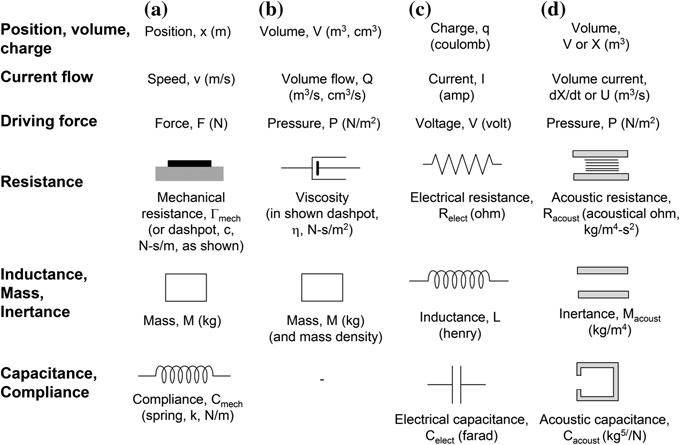
\includegraphics[width=0.7\textwidth]{D1.png}
  \caption{Se muestran los símbolos de los modelos para un modelo a) mecánico, b) de flujo de fluidos, c) eléctrico y d) acústico, junto con los parámetros y unidades comunes para cada uno. El modelo mecánico es para movimiento lineal (rectilíneo). Existen parámetros análogos para el modelo mecánico rotacional, como para un péndulo. La viscosidad también es importante en los modelos mecánicos. Ver también la Tabla~\ref{tab:D1} a continuación (Basado en \cite{D2, D3}).}
  \label{fig:D1}
\end{figure}

En la Fig.~\ref{fig:D2} se muestran los modelos mecánicos, eléctricos y acústicos equivalentes de un sistema típico. El modelo eléctrico se describe mediante

\begin{figure}[htbp]
  \centering
  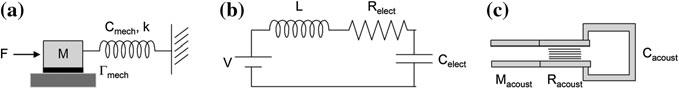
\includegraphics[width=0.8\textwidth]{D2.png}
  \caption{Modelos equivalentes a) mecánicos, b) eléctricos y c) acústicos (Basado en \cite{D2, D3}).}
  \label{fig:D2}
\end{figure}

\begin{equation}
V = L \frac{dI}{dt} + I R + \frac{q}{C}, \label{eq:D.1}
\end{equation}

para un voltaje $V$ que produce una corriente $I$; $I = dq/dt$ donde $q$ es la carga. (Los subíndices específicos para el modelo eléctrico se omiten por simplicidad). Los otros modelos se describen de manera similar, simplemente cambiando los parámetros. La ecuación~\ref{eq:D.1} también se puede escribir como la ecuación diferencial de segundo orden

\begin{equation}
V = L \frac{d^2q}{dt^2} + R \frac{dq}{dt} + \frac{q}{C}, \label{eq:D.2}
\end{equation}

como en (C.30) y (C.34).

La solución general para un voltaje oscilante $V(t) = V_0 \exp(i\omega t)$ es

\begin{equation}
I(t) = \frac{V_0 \exp(i\omega t)}{R + i\omega L + 1/(i\omega C)} = \frac{V(t)}{Z}, \label{eq:D.3}
\end{equation}

con impedancia compleja

\begin{equation}
Z = R + i\omega L + \frac{1}{i\omega C}. \label{eq:D.4}
\end{equation}

La frecuencia de resonancia se observa en la Fig.~\ref{fig:D3} dada por

\begin{SCfigure}[0.75][htbp]
  \centering
  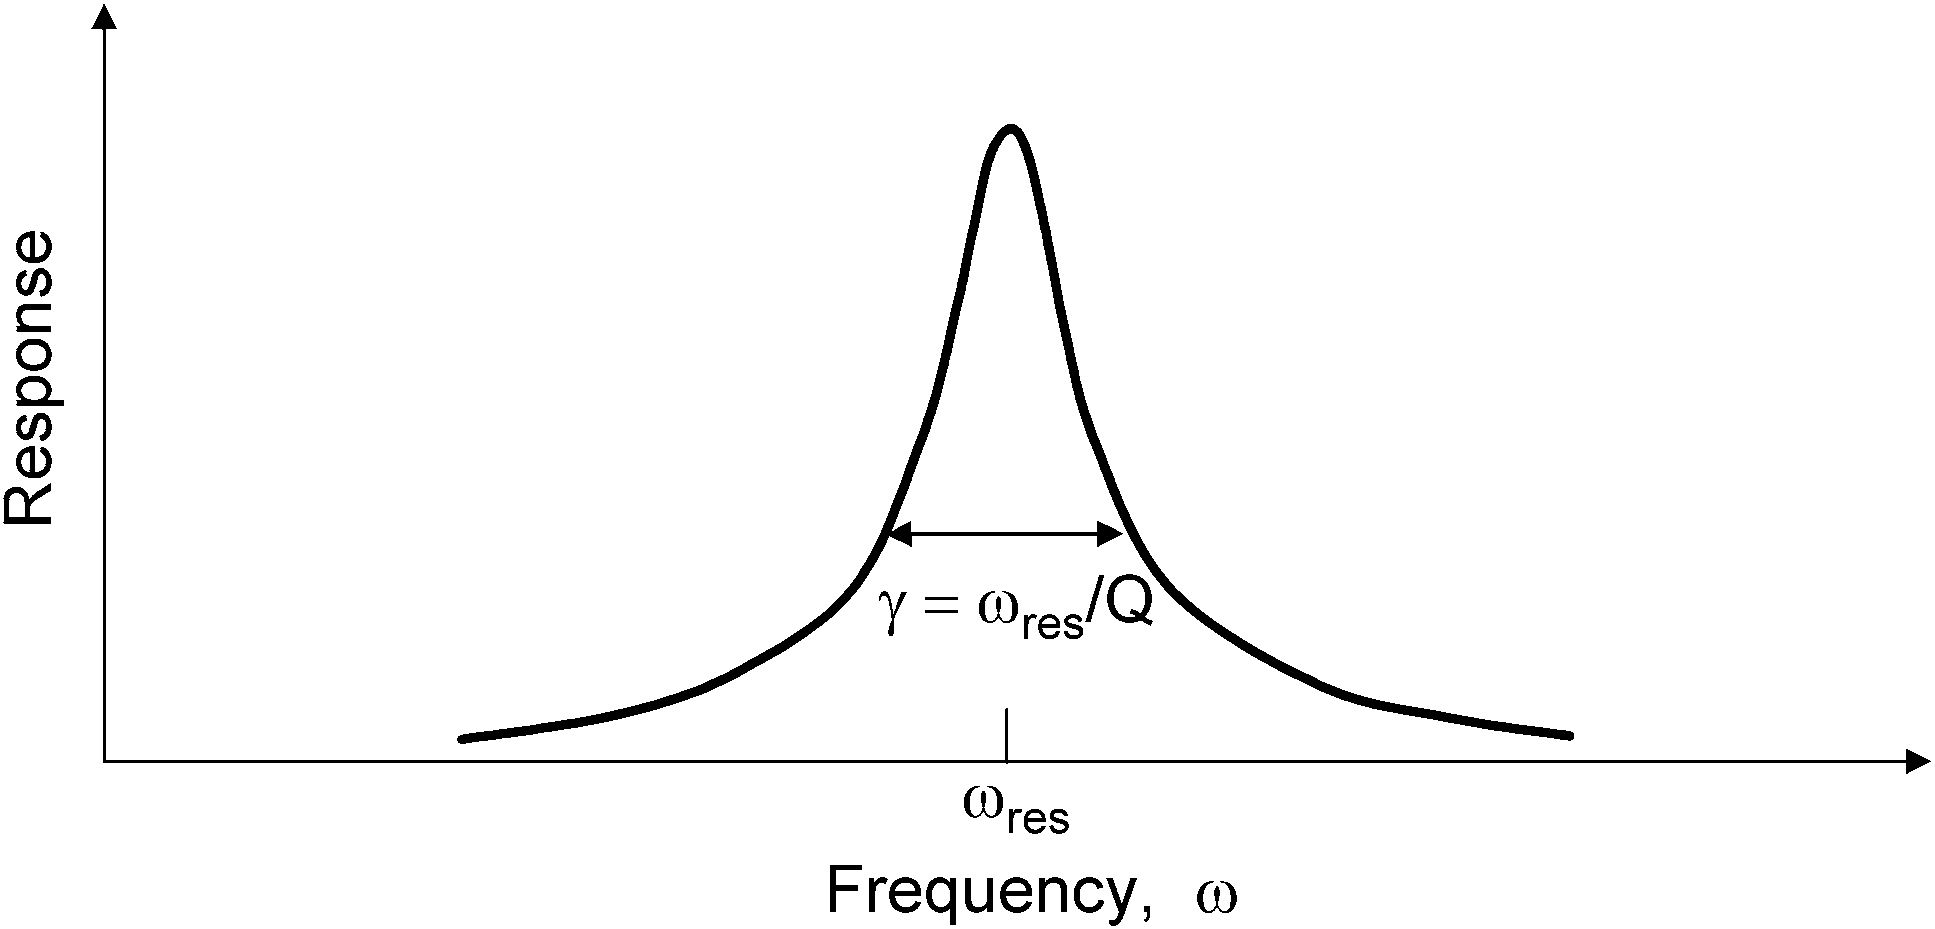
\includegraphics[width=0.6\textwidth]{D3.png}
  \caption{Respuesta resonante.}
  \label{fig:D3}
\end{SCfigure}

\begin{equation}
\omega_{\text{res}} = \frac{1}{\sqrt{LC}} \label{eq:D.5}
\end{equation}

en rad/s y $f_{\text{res}} = 1/(2\pi \sqrt{LC})$ en Hz o cps, y el factor de calidad $Q$ está dado por

\begin{equation}
Q = \frac{\omega_{\text{res}} L}{R}. \label{eq:D.6}
\end{equation}

Utilizando la notación de (C.30) y (C.34)

\begin{equation}
Q = \frac{\omega_{\text{res}}}{\gamma}. \label{eq:D.7}
\end{equation}

El ancho completo de la resonancia (entre los puntos de respuesta a la mitad del máximo) es $\omega_{\text{res}}/Q$, como se ilustra en la Fig.~\ref{fig:D3}. (Este es en realidad el ancho completo solo para resonancias agudas, para las cuales $\omega_{\text{res}} \gg \gamma$ y $Q \gg 1$). Este ancho completo a veces se denomina ancho de banda (cuando se expresa como $f$ en Hz), $\Delta f$, por lo que una definición alternativa de $Q$ es $Q = f/\Delta f$; esta es una definición equivalente en el límite de bajas pérdidas y alto $Q$.

Después de que se apaga la excitación (convirtiéndose (C.34) en (C.30)), la energía en el sistema decae exponencialmente a $1/e$ del valor inicial en un tiempo $t = 1/\gamma = Q/\omega_{\text{res}}$, donde $\gamma$ es la tasa de amortiguamiento (como en (C.30)), que aquí es $R/L$. Este decaimiento ocurre en $Q/2\pi$ períodos de oscilación. Esto es consistente con la definición de $Q$ como $2\pi(\text{energía almacenada})/(\text{energía disipada por ciclo})$.

\section[Análogos Eléctricos del Flujo Sanguíneo]{Modelos distribuidos frente a modelos concentrados: Análogos eléctricos del flujo sanguíneo (Tema avanzado)}
\label{sec:D.1}

Hasta ahora hemos discutido modelos de parámetros concentrados en este apéndice. En (8.2) y (8.11) el flujo se analizó con el vaso como un parámetro «concentrado». También hemos examinado casos en este texto en los que los parámetros están distribuidos por unidad de longitud, como la resistencia al flujo por unidad de longitud para el flujo volumétrico a lo largo de una arteria en el Cap.~8 ((8.14) y (8.15)) y la resistencia eléctrica por unidad de longitud para el flujo de corriente a lo largo de un axón en el Cap.~12 ((12.60) y (12.67)). Estos son modelos «distribuidos» o de «línea de transmisión».

En la Fig.~12.17 se muestra una versión discretizada del modelo eléctrico distribuido. Digamos que cada sección repetida tiene una longitud (muy corta) $\Delta x$. Los cambios en el voltaje eléctrico (la fuerza impulsora) y la corriente (la respuesta) (Tabla~\ref{tab:D1}) a lo largo de esta longitud de un cable eléctrico se describen mediante [566, 861]

\begin{equation}
V_{\text{elect}}(x) - V_{\text{elect}}(x + \Delta x) = -\frac{\partial V_{\text{elect}}}{\partial x} \Delta x = L_{\text{elect}} \frac{\partial I}{\partial t} + I R_{\text{elect}} \label{eq:D.8}
\end{equation}

\begin{equation}
I(x) - I(x + \Delta x) = -\frac{\partial I}{\partial x} \Delta x = C_{\text{elect}} \frac{\partial V_{\text{elect}}}{\partial t} + \frac{V_{\text{elect}}}{R_{\text{elect}}}. \label{eq:D.9}
\end{equation}

$V_{\text{elect}}$ e $I$ son funciones de $x$ y $t$. La resistencia, inductancia y capacitancia son aquellas correspondientes a esta longitud $\Delta x$, y también pueden variar con $x$. Estas ecuaciones se pueden obtener utilizando las leyes de Kirchhoff (la segunda y primera ley, respectively). Se derivaron y luego se combinaron en la discusión de señales eléctricas a lo largo de los nervios en el Cap.~12 (Fig.~12.17) para dar las ecuaciones del telégrafo. Parte de la primera ecuación es la ley de Ohm, con la caída de voltaje $\Delta V_{\text{elect}} = -(\partial V_{\text{elect}}/\partial x)\Delta x = I R_{\text{elect}}$.

Las ecuaciones análogas para el flujo sanguíneo a lo largo de un vaso de longitud $\Delta x$ son:

\begin{equation}
P(x) - P(x + \Delta x) = -\frac{\partial P}{\partial x} \Delta x = L_{\text{flow}} \frac{\partial Q}{\partial t} + Q R_{\text{flow}} \label{eq:D.10}
\end{equation}

\begin{equation}
Q(x) - Q(x + \Delta x) = -\frac{\partial Q}{\partial x} \Delta x = C_{\text{flow}} \frac{\partial P}{\partial t} + \frac{P}{R_{\text{flow}}} \label{eq:D.11}
\end{equation}

\begin{table}[htbp]
\centering
\caption{Análogo del flujo sanguíneo y circuitos eléctricos (con unidades).}
\label{tab:D1}
\begin{tabularx}{\textwidth}{>{\hsize=1.0\hsize}X >{\hsize=1.0\hsize}X}
\toprule
\textbf{Parámetro de circulación sanguínea} & \textbf{Parámetro eléctrico} \\
\midrule
Volumen, $V_{\text{flow}}$ ($\text{m}^3$) & Carga, $q$ (C, coulomb) \\
Tasa de flujo sanguíneo, $Q$ ($\text{m}^3/\text{s}$) & Corriente, $I$ (A, amperio) \\
Presión, $P$ ($\text{N}/\text{m}^2$) & Voltaje, $V_{\text{elect}}$ (V, voltio) \\
Resistencia vascular, $R_{\text{flow}}$ ($\text{N}\cdot\text{s}/\text{m}^5$) & Resistencia, $R_{\text{elect}}$ ($\Omega$, ohmio) \\
Inertancia, $L_{\text{flow}}$ ($\text{kg}/\text{m}^4$) & Inductancia, $L_{\text{elect}}$ (H, henrio) \\
Distensibilidad, $C_{\text{flow}}$ ($\text{m}^5/\text{N}\cdot\text{s}$) & Capacitancia, $C_{\text{elect}}$ (F, faradio) \\
\bottomrule
\end{tabularx}
\end{table}

donde ahora la presión es la fuerza impulsora para la tasa de flujo sanguíneo $Q$ y $R_{\text{flow}}$ es la resistencia vascular. Sin el término de inertancia, la primera ecuación es simplemente la ley de Poiseuille (7.25), con la caída de presión $\Delta P = -(\partial P/\partial x)\Delta x = Q R_{\text{elect}}$. Los parámetros de flujo son

\begin{equation}
R_{\text{flow}} = \frac{8\pi\eta L}{A^2} \label{eq:D.12}
\end{equation}

\begin{equation}
C_{\text{flow}} = \frac{3L A(1 + r/w)^2}{Y(1 + 2r/w)} \label{eq:D.13}
\end{equation}

\begin{equation}
L_{\text{flow}} = \frac{\rho L}{A}, \label{eq:D.14}
\end{equation}

donde $A$ es el área de la sección transversal del vaso, $L$ es su longitud (que es $\Delta x$ para el modelo discretizado), $r$ es su radio, $w$ es el espesor de su pared y $\rho$ es la densidad de masa de la sangre. Estas ecuaciones son útiles para rastrear el flujo sanguíneo dentro de vasos con propiedades tanto resistivas como de distensibilidad.

Todos los modelos de materiales (y sistemas y procesos) pueden mejorarse matemáticamente añadiendo más términos, como en el modelo mecánico de la Fig.~5.13. Las cuestiones más importantes son si los elementos en tales modelos simples o más complejos corresponden a los componentes físicos del material. Incluso si no lo hacen, sigue siendo importante saber si el modelo se puede utilizar para predecir el funcionamiento correctamente cuando se cambian las condiciones.

\begin{thebibliography}{99}
\bibitem{D1} G.N. Jager, N. Westerhof, A. Noordergraaf, Oscillatory flow impedance in electrical analog of arterial system: representation of sleeve effect and non-Newtonian properties of blood. \textit{Circ. Res.} \textbf{16}, 121--133 (1965)
\bibitem{D2} H.F. Olson: \textit{Acoustical Engineering} (Van Nostrand, Princeton, 1957)
\bibitem{D3} H.F. Olson: \textit{Music, Physics, and Engineering}, 2.ª ed. (Dover, Nueva York, 1967)
\end{thebibliography}


% ---- Apéndice E: Biofísica del cuerpo humano ----

\chapter{Biofísica del cuerpo humano}
\label{ch:appendixE}

Este apéndice ubica los contenidos de este texto dentro del campo de la biofísica. La biofísica es difícil de definir bien, como lo ilustran las muchas definiciones definitivas pero diferentes de biofísica proporcionadas en \cite{E1,E2,E3,E4,E5,E6,E7,E8,E9,E10,E11,E12}. En términos generales, la biofísica es la aplicación de la física y los principios físicos a la biología. En este contexto, virtualmente todo lo presentado en este libro es biofísica. Sin embargo, este término a menudo se utiliza en el sentido más restringido del uso de la física a un nivel más molecular y celular. Utilizaremos este contexto más estrecho durante el resto de este apéndice, y en este sentido restringido muchos temas cubiertos aquí siguen siendo biofísica, pero muchas áreas de la biofísica no han sido cubiertas. Otra definición más de biofísica es el estudio de la biología utilizando métodos físicos. Esto se distingue de la física biológica, que es el estudio de las propiedades físicas de la biología.

Un tema en biofísica es la estructura molecular de los sistemas biológicos. Esto incluye la electrostática de los iones en soluciones (Cap.~12), la estructura de las biomacromoléculas, tales como las proteínas, y áreas como el plegamiento de proteínas, la estructura y las propiedades de las interfaces entre medios biológicos como las membranas celulares (tensión superficial en los Caps.~7 y 9, membranas de células nerviosas en el Cap.~12) y los canales iónicos en las membranas (que se tocan muy brevemente en la conducción nerviosa en el Cap.~12).

La mecánica estadística es el examen de sistemas compuestos por muchos objetos o sistemas similares, cada uno de los cuales está bien caracterizado. Todo el conjunto de sistemas a menudo está en equilibrio térmico y, tras el análisis de la mecánica estadística, puede tratarse utilizando la termodinámica. El tratamiento de los iones en solución en el Cap.~12 es el resultado de la mecánica estadística. Como se indicó en el Cap.~5, la curva de fuerza-velocidad de Hill de los músculos se puede derivar del análisis de la mecánica estadística de los numerosos puentes cruzados de actina-miosina (lo cual no se hizo aquí). Muchos aspectos de las membranas celulares y de la estructura de las proteínas ---como el plegamiento--- se pueden examinar utilizando métodos de mecánica estadística.

La biofísica incluye la bioenergética del proceso de fotosíntesis y la síntesis de ATP y su uso. En el Cap.~6 examinamos la biofísica del uso de la energía en el cuerpo humano. El movimiento de los organismos, como el movimiento de las bacterias y el movimiento muscular, forman parte de la biofísica molecular y celular; la base microscópica del funcionamiento muscular se exploró en el Cap.~5. Las propiedades electroquímicas de las membranas celulares y las señales nerviosas, tal como se discute en el Cap.~12, siempre han sido temas centrales en biofísica. Algunos incluyen dentro de la biofísica la integración de nivel superior y las combinaciones de sistemas moleculares y celulares, como la memoria, el control del movimiento, la integración visual, y la conciencia y el pensamiento.

El uso de la caracterización física en problemas biológicos juega un papel central en la biofísica, como el uso de la difracción de rayos X (XRD) para determinar la estructura molecular, la resonancia magnética nuclear (NMR) para estudiar moléculas en entornos más naturales de lo que permite la difracción de rayos X, la microscopía de efecto túnel (STM) para examinar la estructura atómica de las superficies, la microscopía de fuerza atómica (AFM) para examinar superficies y medir fuerzas, y las pinzas ópticas para manipular moléculas. Tanto el AFM como las pinzas ópticas han sido fundamentales para estudiar las interacciones fundamentales en los músculos, como los puentes cruzados individuales de actina-miosina (Cap.~5).

\begin{thebibliography}{99}
\bibitem{E1} R.M.J. Cotterill, \textit{Biophysics: An Introduction} (Wiley, Nueva York, 2002)
\bibitem{E2} M. Daune, \textit{Molecular Biophysics: Structures in Motion} (Oxford University Press, Oxford, 1999)
\bibitem{E3} R. Glaser, \textit{Biophysics} (Springer, Berlín, 2000)
\bibitem{E4} R.E. Goldstein, P.C. Nelson, T.R. Powers, Teaching biological physics. \textit{Phys. Today} \textbf{58}(3), 46--51 (2005)
\bibitem{E5} F.R. Hallett, R.H. Stinson, P.A. Speight, \textit{Physics for the Biological Sciences: A Topical Approach to Biophysical Concepts} (Methuen/Chapman \& Hall, Toronto, 1982)
\bibitem{E6} P. Maróti, L. Berkes, F. Tölgyesi, \textit{Biophysics Problems: A Textbook with Answers} (Akadémiai Kiadó, Budapest, 1998)
\bibitem{E7} H.J. Metcalf, \textit{Topics in Classical Biophysics} (Prentice-Hall, Englewood Cliffs, 1980)
\bibitem{E8} P. Nelson, \textit{Biological Physics: Energy, Information, Life} (Freeman, Nueva York, 2003)
\bibitem{E9} B. Nolting, \textit{Methods in Modern Biophysics} (Springer, Berlín, 2003)
\bibitem{E10} R. Phillips, S.R. Quake, The biological frontier of physics. \textit{Phys. Today} \textbf{59}(5), 38--43 (2006)
\bibitem{E11} R.B. Setlow, E.C. Pollard, \textit{Molecular Biophysics} (Addison-Wesley, Reading, 1962)
\bibitem{E12} M.P. Sheetz (ed.), \textit{Laser Tweezers in Cell Biology}, Methods in Cell Biology, Vol. 55 (Academic, San Diego, 1998)
\end{thebibliography}

% Control de Calidad: 46 párrafos origen -> 46 párrafos salida. Mapeo 1:1 verificado. Sin omisiones.

% ==================== APÉNDICES F Y G ====================
\chapter[Física de los Ciclos de Vida]{Física de los ciclos de vida: embarazo, lesiones, enfermedades y trastornos, envejecimiento y muerte}
\label{app:f}

Este apéndice ofrece una visión general de la física del cuerpo descrita a lo largo del texto para condiciones especiales. Cada sección comienza haciendo referencia a ejemplos relevantes en los capítulos del texto y continúa describiendo cómo utilizar el índice para encontrar estas discusiones.

\section{Embarazo}
\label{sec:f1}

La física de diversas características del embarazo, el parto y los recién nacidos descrita en el texto incluye cómo el equilibrio de la futura madre se ve afectado por los cambios en la masa corporal (en el cap.~2) y la estructura de las vértebras de las mujeres (cap.~2), cómo se ablanda el cuello uterino a medida que se acerca el parto (cap.~4), cómo crecen los músculos en el feto (cap.~5), cómo aumenta la tasa metabólica de la futura madre debido al incremento de sus propias necesidades metabólicas y a la necesidad de formar el feto, la placenta, etcétera (cap.~6), las necesidades de circulación sanguínea de la futura madre y del feto (cap.~8), las necesidades respiratorias de la madre (cap.~9) y cómo el embarazo es un proceso de retroalimentación positiva en el cuerpo (cap.~13).

Consulte la entrada «Embarazo» en el índice para todas las referencias al embarazo, el parto y el recién nacido.

\section{Lesiones}
\label{sec:f2}

Se discuten las ventajas de usar bastones y tener reemplazos de cadera para recuperarse de algunas lesiones, así como el dolor lumbar y las dislocaciones de hombro (en el cap.~2). Se analizan las lesiones que pueden resultar de colisiones, incluidas aquellas que pueden ocurrir durante eventos atléticos y en automóviles (cap.~3). Se abordan los daños a los componentes estructurales del cuerpo, como los debidos a fracturas óseas y daños en los tendones, y cómo evitar tales daños, junto con los tipos de lesiones que pueden ocurrir durante eventos deportivos (cap.~4).

Consulte la entrada «Lesiones» en el índice para todas las referencias a lesiones físicas generales, y «Lesiones deportivas» para aquellas que comúnmente resultan de eventos atléticos. Para lesiones en los ojos, aquellas debidas a descargas eléctricas y similares, busque bajo «Enfermedades y trastornos».

\section{Enfermedades y trastornos}
\label{sec:f3}

A lo largo del texto se hacen referencias a los aspectos físicos de diversas enfermedades y trastornos, incluyendo conmociones cerebrales y otros tipos de daños debidos a colisiones de la cabeza (en el cap.~3), enfermedades y trastornos cardíacos y circulatorios, tales como el endurecimiento de las arterias, insuficiencia cardíaca, arritmias, ataques isquémicos transitorios y aneurismas (cap.~8), trastornos respiratorios (cap.~9), modos de pérdida auditiva debido a trastornos médicos y patologías del oído medio (cap.~10), afecciones relacionadas con la visión, tales como la formación de cataratas, desprendimiento o enfermedad de la retina, glaucoma, queratocono, daltonismo y alteración de la agudeza visual (cap.~11), y los efectos de las descargas eléctricas (cap.~12).

Consulte la entrada «Enfermedades y trastornos» en el índice para referencias a enfermedades, trastornos generales, lesiones distintas de aquellas en los componentes estructurales que ocurren durante movimientos comunes (en los ojos, el sistema nervioso, etcétera), los efectos de las balas, etcétera.

Se abordan los trastornos y las condiciones graves o inusuales que experimentan los astronautas durante y después de los vuelos espaciales, incluyendo cómo cambian sus cuerpos (cap.~1), el «caminar lunar» y el efecto de la aceleración sostenida (cap.~3), y el volumen de sonido alto durante el despegue (cap.~10).

Observamos que muchos consideran que algunas enfermedades y trastornos son resultado en gran medida de factores ambientales de la vida humana moderna, tales como la diabetes tipo 2, el dolor lumbar (cap.~2), la hipertensión y las enfermedades cardíacas (cap.~8), la miopía (cap.~11), etcétera; a menudo se les denomina enfermedades de desajuste (no infecciosas)~\cite{f7}.

\section{Envejecimiento}
\label{sec:f4}

Las características del envejecimiento descritas en el texto se relacionan con los aspectos físicos de la fisiología. A medida que se avanza en edad, se puede necesitar un bastón para mantener la estabilidad o prevenir el dolor al estar de pie o al caminar (en el cap.~2). Se camina y se corre más lento, con zancadas más cortas (cap.~3). La densidad ósea disminuye (osteoporosis) y los umbrales de fractura en los huesos disminuyen debido a esto y a la acumulación de microfisuras y tensiones; las propiedades de los materiales de otros componentes estructurales también empeoran (cap.~4). Pueden ser necesarios reemplazos de cadera debido al daño acumulado (problemas del cap.~4). La forma de las vértebras cambia, lo que conduce a una disminución de la estatura, a la flexión hacia adelante de la columna vertebral y a una postura encorvada. La masa muscular general disminuye y la fuerza decae debido a esto y a factores neuronales; el porcentaje de fibras de contracción rápida en los músculos disminuye y las reacciones se vuelven más lentas (cap.~5). El rendimiento máximo incluso de personas muy entrenadas en carrera y natación disminuye, al igual que las tasas metabólicas basales (cap.~6), lo que, junto con un estilo de vida menos activo, puede provocar un aumento del peso corporal (debido a que el incremento en la masa de grasa corporal compensa con creces la disminución de la masa muscular, y con esto la forma del cuerpo se vuelve más endomórfica) (cap.~1). (La buena noticia es que entonces se vuelve más fácil para el cuerpo flotar (cap.~7)). Sin embargo, las personas mayores de 70 años a menudo pierden peso~\cite{f17}.

Con el avance de la edad, la presión arterial suele aumentar y la placa se acumula en las arterias, lo que puede provocar enfermedades cardíacas; la frecuencia cardíaca máxima recomendada disminuye, y el gasto cardíaco, el volumen sistólico y la frecuencia cardíaca disminuyen (cap.~8). El consumo de oxígeno y la diferencia de oxígeno arterial y venoso disminuyen (cap.~9). La audición empeora a medida que aumentan los niveles de umbral auditivo (presbiacusia) y la voz envejece (presbifonía) con aumentos en el tono y el temblor, etcétera (cap.~10). La capacidad del cristalino del ojo para acomodarse a enfocar objetos tanto cercanos como lejanos disminuye (presbicia), y aumenta la probabilidad de enfermedades y trastornos oculares, incluyendo que el cristalino se vuelva opaco a medida que se desarrollan cataratas (cap.~11). Los tiempos de reacción aumentan y los reflejos empeoran, en parte debido a tiempos de reacción nerviosa más lentos, y nuestra capacidad de equilibrio empeora (cap.~12). Finalmente, a medida que los componentes del sistema circulatorio fallan notablemente, los sistemas de retroalimentación y control del cuerpo pueden acelerar las etapas finales del proceso de muerte (cap.~13).

Aunque la mayoría de estas características asociadas con el envejecimiento pueden no parecer muy atractivas, en el lado positivo el envejecimiento conduce a una mayor base de experiencia y sabiduría, y a algo más que el autor no es capaz de recordar en este momento.

Consulte la entrada «Envejecimiento» en el índice para ver todas las referencias al envejecimiento.

Se puede encontrar más información sobre el envejecimiento en la revisión general~\cite{f8} y en revisiones de las teorías del envejecimiento~\cite{f16} y de la biología y fisiología del envejecimiento~\cite{f1, f11}, así como en revisiones enfocadas en el rendimiento de atletas veteranos~\cite{f13, f14}, precisión del movimiento~\cite{f2}, pérdida ósea (osteoporosis)~\cite{f9}, la matriz extracelular~\cite{f12}, rendimiento muscular (lo que se denomina sarcopenia)~\cite{f3}, balance energético~\cite{f17}, rendimiento en natación~\cite{f4}, el sistema cardiovascular~\cite{f5}, función pulmonar~\cite{f10, f15} y regulación de la temperatura~\cite{f6}.

\section{Muerte}
\label{sec:f5}

En el texto se señalan algunos aspectos de la muerte, incluyendo la probabilidad de fatalidad durante un traumatismo craneoencefálico debido a choques de automóviles, boxeo, etcétera (cap.~3), afecciones cardíacas fatales (cap.~8), muerte por descargas eléctricas (cap.~12) y un modo común de muerte en personas muy ancianas que es promovido por la retroalimentación positiva en el cuerpo (cap.~13).

El texto también cubre áreas relacionadas con «La regla de los tres», que es una guía muy aproximada para la supervivencia antes de morir. Se puede sobrevivir 3~min sin aire (sin respirar debido a ahogamiento o asfixia, cap.~9) (y también 3~min en agua helada, Fig.~6.22), 3~h sin refugio (con exposición extrema, cap.~6), 3 días sin agua (deshidratación) y 3 semanas sin comida (inanición, pero con agua y refugio adecuados, Fig.~6.14). Los límites extremos antes de la muerte pueden ser más cortos o más largos para una persona y condiciones dadas.

Consulte la entrada «Muerte» en el índice para todas las referencias al proceso de morir; también es posible que desee buscar bajo «Enfermedades y trastornos».

\begin{thebibliography}{99}
\bibitem{f1} I. B. Abrass, The biology and physiology of aging. W. J. Med. \textbf{153}, 641--645 (1990)
\bibitem{f2} E. A. Christou, M. Shinohara, R. M. Enoka, Fluctuations in acceleration during voluntary contractions lead to greater impairment of movement accuracy in old adults. J. Appl. Physiol. \textbf{95}, 373--384 (2003)
\bibitem{f3} T. J. Doherty, Invited review: aging and sarcopenia. J. Appl. Physiol. \textbf{95}, 1717--1727 (2003)
\bibitem{f4} A. J. Donato, K. Tench, D. H. Glueck, D. R. Seals, I. Eskurza, H. Tanaka, Declines in physiological functional capacity with age: a longitudinal study in peak swimming performance. J. Appl. Physiol. \textbf{94}, 764--769 (2003)
\bibitem{f5} A. U. Ferrari, A. Radaelli, M. Centola, Invited review: aging and the cardiovascular system. J. Appl. Physiol. \textbf{95}, 2591--2597 (2003)
\bibitem{f6} W. L. Kenney, T. A. Munce, Invited review: aging and human temperature regulation. J. Appl. Physiol. \textbf{95}, 2598--2603 (2003)
\bibitem{f7} D. E. Lieberman, \emph{The Story of the Human Body: Evolution, Health, and Disease} (Pantheon, Nueva York, 2013)
\bibitem{f8} D. L. Longo, A. S. Fauci, D. L. Kasper, S. L. Hauser, J. Jameson, J. Loscalzo (eds.), \emph{Harrison's Principles of Internal Medicine}, 18.ª~ed. (McGraw-Hill, Nueva York, 2011)
\bibitem{f9} E. Seeman, Invited review, Pathogenesis of osteoporosis. J. Appl. Physiol. \textbf{95}, 2142--2151 (2003)
\bibitem{f10} G. Sharma, J. Goodwin, Effect of aging on respiratory system physiology and immunology. Clin. Interventions Aging \textbf{1}, 253--260 (2006)
\bibitem{f11} G. C. Sieck, Physiology of aging. J. Appl. Physiol. \textbf{95}, 1333--1334 (2003)
\bibitem{f12} F. H. Silver, D. DeVore, L. M. Siperko, Invited review: role of mechanophysiology in aging of ECM: effects of changes in mechanochemical transduction. J. Appl. Physiol. \textbf{95}, 2134--2141 (2003)
\bibitem{f13} H. Tanaka, D. R. Seals, Invited review: dynamic exercise performance in masters athletes: insight into the effects of primary human aging on physiological functional capacity. J. Appl. Physiol. \textbf{95}, 2152--2162 (2003)
\bibitem{f14} H. Tanaka, D. R. Seals, Topical review: endurance exercise performance in Masters athletes: age-associated changes and underlying physiological mechanisms. J. Physiol. \textbf{586}, 55--63 (2008)
\bibitem{f15} W. M. Wahba, Influence of aging on lung function-clinical significance of changes from age twenty. Anesth. Analg. \textbf{62}, 764--776 (1983)
\bibitem{f16} B. T. Weinert, P. S. Timiras, Theories of aging. J. Appl. Physiol. \textbf{95}, 1706--1716 (2003)
\bibitem{f17} M.-M. G. Wilson, J. E. Morley, Invited review: aging and energy balance. J. Appl. Physiol. \textbf{95}, 1728--1736 (2003)
\end{thebibliography}

\chapter{Física de los deportes}
\label{app:g}

Muchos de los movimientos importantes en los deportes se analizan en los caps.~3 y 7 utilizando física simple. Esto incluye el movimiento real del cuerpo al lanzar una pelota o golpearla con un bate o una raqueta, el vuelo de la pelota y las colisiones. Otros capítulos abordan aspectos adicionales de las actividades deportivas, tales como lesiones y cascos (en el cap.~4), la acción de los músculos (cap.~5), el aumento de las tasas metabólicas y la necesidad de enfriamiento corporal (cap.~6), y el aumento de las frecuencias respiratorias (cap.~9). Como tal, este apéndice aborda aspectos importantes de la física realizada por el cuerpo. Además, hemos examinado más específicamente la física de varios deportes, incluidos el atletismo de pista y campo, el béisbol y el boxeo.

Existen varios libros dedicados a la física de los deportes; algunos se centran en un solo deporte y otros examinan varios de ellos. Algunos enfatizan el objeto del deporte y no cómo el cuerpo humano genera la acción necesaria. (No obstante, son muy interesantes). El excelente libro de Hay~\cite{g17} es una de las varias excepciones, ya que examina la biomecánica de many sports, incluyendo la gimnasia, la natación, el atletismo y varios deportes de equipo importantes. Igualmente excelente es la perspicaz descripción general de Brancazio~\cite{g4}, que describe la física de las muchas características de las actividades deportivas de manera simple, pero precisa y completa. La revisión general de Dyson~\cite{g10} enfatiza áreas que no siempre son cubiertas por otros, tales como la gimnasia y los eventos de atletismo. Otras buenas revisiones generales de muchos deportes se pueden encontrar en~\cite{g27}.

Se puede encontrar un excelente compendio de artículos que describen muchos deportes en el libro de Armenti~\cite{g3}, incluyendo aquellos sobre tiro con arco, bádminton, béisbol, baloncesto, bolos, piragüismo, ciclismo, lanzamiento de disco, saltos, fútbol americano, golf, saltos, karate, remo, carrera, vela, lanzamiento de peso, esquí, natación y tenis. La mayoría se centra en los movimientos mismos, pero algunos se enfocan en el metabolismo. Se puede obtener una buena noción del alcance de la física en el atletismo leyendo detenidamente estos artículos o los libros citados de Brancazio, Dyson y Hay. En~\cite{g13, g14} se pueden encontrar bibliografías completas de artículos y otros recursos sobre la física de los deportes.

El libro editado por Hung y Pallis~\cite{g18} examina la física del golf, el tenis, el béisbol, el fútbol americano y el fútbol (soccer), y el baloncesto. Adair~\cite{g1, g2} y Watts y Bahill~\cite{g28} han analizado el béisbol, concentrándose en el movimiento de la pelota durante un lanzamiento y después de haber sido golpeada. Otros libros y artículos valiosos sobre el béisbol incluyen~\cite{g7, g25}.

Gay~\cite{g15} discute la física del fútbol americano. La física del baloncesto está cubierta en~\cite{g12} y la del tenis en~\cite{g5}. Varios aspectos del ciclismo están cubiertos en~\cite{g6}; Brancazio~\cite{g4} presenta una buena discusión sobre la estabilidad de las bicicletas. Jorgensen~\cite{g19} ha examinado el golf. El golf también se destaca en el libro de~\cite{g8}. Lind y Sanders~\cite{g24} han analizado la física del esquí, incluyendo el movimiento de esquí, la nieve, la cera para esquís, etcétera.

Los vuelos de las pelotas y otros proyectiles se cubren en~\cite{g4, g7, g8, g16, g26}. En particular, los libros de Daish~\cite{g8} y de Mestre~\cite{g9} resuelven la física a un alto nivel. El primer libro es un poco más completo, mientras que el segundo aborda algunos problemas más difíciles.

Los libros de Laws y colaboradores~\cite{g11, g20, g21, g22, g23} examinan un tema relacionado con la física de los deportes: la física de la danza.

Las discusiones del texto sobre los siguientes deportes, movimientos y equipos deportivos se pueden localizar a partir de los siguientes listados en el índice: Tiro con arco y flechas; Pelotas; Béisbol; Baloncesto; Bateo; Bicicleta; Navegación; Rebote; Bolos; Boxeo; Transporte; Recepción; Escalar, subir, bajar escaleras; Críquet; Ciclismo; Danza; Clavados; Ejercicio; Fútbol americano; Vuelo, vuelo humano; Golf; Gimnasia; Lanzamiento de martillo; Salto de altura; Hockey; Saltos cortos; Saltos; Karate; Patadas; Levantamiento; Salto de longitud; Carrera de maratón; Ping-pong, tenis de mesa; Lanzamiento (picheo); Salto con pértiga; Billar; Tirar, empujar; Flexiones; Marcha atlética; Pelota rodante; Carrera; Palear; Lanzamiento de peso; Estar sentado; Patinaje; Pelota derrapando; Esquí; Saltar a la comba; Deslizarse; Resbalarse; Fútbol; Volteretas; Pelota giratoria; Lesiones deportivas; Sprint; Escaleras; Estar de pie; Golpear, pegar, puñetazos; Natación; Balanceo; Tenis; Lanzamiento; Cinta de correr; Salto vertical; Caminar; Levantamiento de pesas, entrenamiento; y Lucha libre.

Consulte «Lesiones deportivas» en el índice para ver las lesiones resultantes de eventos atléticos.

\begin{thebibliography}{99}
\bibitem{g1} R. K. Adair, \emph{The Physics of Baseball}, 3.ª~ed. (HarperCollins, Nueva York, 2002)
\bibitem{g2} R. K. Adair, The physics of baseball. Phys. Today 26--31 (1995)
\bibitem{g3} A. Armenti Jr. (ed.), \emph{The Physics of Sports}, American Institute of Physics (Springer, Nueva York, 1992)
\bibitem{g4} P. J. Brancazio, \emph{Sport Science: Physical Laws and Optimum Performance} (Touchstone, Nueva York, 1984)
\bibitem{g5} H. Brody, R. Cross, C. Lindsey, \emph{The Physics and Technology of Tennis} (Usrsa, Vista, California, 2004)
\bibitem{g6} E. R. Burke (ed.), \emph{Science of Cycling} (Human Kinetics, Champaign, Illinois, 1986)
\bibitem{g7} R. Cross, \emph{Physics of Baseball and Softball} (Springer, Nueva York, 2011)
\bibitem{g8} C. B. Daish, \emph{The Physics of Ball Games} (The English Universities Press, Londres, 1972)
\bibitem{g9} N. de Mestre, \emph{The Mathematics of Projectiles in Sport} (Cambridge University Press, Cambridge, 1990)
\bibitem{g10} G. H. G. Dyson, B. D. Woods, P. R. Travers, \emph{Dyson's Mechanics of Athletics}, 8.ª~ed. (Holmes \& Meier, Nueva York, 1986)
\bibitem{g11} S. S. Fitt, \emph{Dance Kinesiology}, 2.ª~ed. (Schirmer/Thomson Learning, Nueva York, 1996)
\bibitem{g12} J. J. Fontanella, \emph{The Physics of Basketball} (The Johns Hopkins University Press, Baltimore, 2006)
\bibitem{g13} C. Frohlich, Resource letter PS-1: physics of sports. Am. J. Phys. \textbf{54}, 590--593 (1986)
\bibitem{g14} C. Frohlich, Resource letter PS-2: physics of sports. Am. J. Phys. \textbf{79}, 565--574 (2011)
\bibitem{g15} T. Gay, \emph{The Physics of Football: Discover the Science of Bone-Crunching Hits, Soaring Field Goals, and Awe-Inspiring Passes} (HarperCollins, Nueva York, 2005)
\bibitem{g16} D. F. Griffing, \emph{The Dynamics of Sports: Why That's the Way the Ball Bounces}, 4.ª~ed. (Dalog, Oxford, Ohio, 1995)
\bibitem{g17} J. G. Hay, \emph{The Biomechanics of Sports Techniques}, 4.ª~ed. (Prentice-Hall, Englewood Cliffs, 1993)
\bibitem{g18} G. K. Hung, J. M. Pallis (eds.), \emph{Biomedical Engineering Principles in Sports} (Kluwer/Plenum, Nueva York, 2004)
\bibitem{g19} T. P. Jorgensen, \emph{The Physics of Golf}, 2.ª~ed. (AIP/Springer, Nueva York, 1999)
\bibitem{g20} K. Laws, \emph{The Physics of Dance} (Schirmer Books, Nueva York, 1984)
\bibitem{g21} K. Laws, C. Harvey, M. Swope, \emph{Physics, Dance, and the Pas De Deux} (Schirmer Books, Nueva York, 1994)
\bibitem{g22} K. Laws, M. Swope, \emph{Physics and the Art of Dance: Understanding Movement} (Oxford University Press, Oxford, 2002)
\bibitem{g23} K. Laws, M. Lott, Resource letter PoD-1: physics of dance. Am. J. Phys. \textbf{81}, 7--13 (2013)
\bibitem{g24} D. Lind, S. P. Sanders, \emph{The Physics of Skiing: Skiing at the Triple Point} (AIP/Springer, Nueva York, 1996)
\bibitem{g25} A. M. Nathan, L. V. Smith, W. L. Faber, D. A. Russell, Corked bats, juiced balls, and humidors: the physics of cheating in baseball. Am. J. Phys. \textbf{79}, 575--580 (2011)
\bibitem{g26} M. S. Townend, \emph{Mathematics in Sport} (Ellis Horwood Ltd, West Sussex, 1984)
\bibitem{g27} F. Vizard (ed.), \emph{Why a Curveball Curves: The Incredible Science of Sports (Popular Mechanics)} (Hearst, Nueva York, 2009)
\bibitem{g28} R. G. Watts, A. T. Bahill, \emph{Keep Your Eye on the Ball: Curve Balls, Knuckleballs, and Fallacies of Baseball} (Freeman, Nueva York, 2000)
\end{thebibliography}

% Control de Calidad: 81 párrafos origen -> 81 párrafos salida. Mapeo 1:1 verificado. Sin omisiones.

% ==================== APÉNDICE H ====================
\chapter[Mediciones, Imágenes y Tratamiento]{Física para el cuerpo: mediciones, imágenes y tratamiento}\label{ch:appendixH}

Este apéndice aborda la física aplicada al cuerpo. Comienza con una breve descripción general de la física de las mediciones y los tratamientos médicos que utilizan luz, ultrasonido, rayos X, radiactividad e imágenes por resonancia magnética. Concluye con localizadores de temas sobre la física de las mediciones y del tratamiento que se presentan en el texto principal. Hay relativamente pocos ejemplos de este tipo porque este no es el énfasis de este libro.

Esta área de la física dedicada al diagnóstico y tratamiento de enfermedades se conoce en los Estados Unidos como «física médica» \cite{H2}. Algunos la subdividen en radiología diagnóstica y terapéutica, medicina nuclear diagnóstica y terapéutica, ultrasonido, imágenes por resonancia magnética y las aplicaciones de láseres para el diagnóstico y tratamiento \cite{H2}, y otros, de una manera ligeramente diferente, en física de la radioterapia, física de la obtención de imágenes, física de la medicina nuclear y física de la salud \cite{H4}. La física médica se aborda en \cite{H3} y muchos recursos en esta área se enumeran en \cite{H1, H2}. Los recursos para el área más restringida de la radioterapia se pueden encontrar en \cite{H4}.

\section{Descripción general}\label{sec:H1}

La luz visible se utiliza ampliamente para la inspección médica, y la luz visible y ultravioleta se utilizan ampliamente para el tratamiento médico. Las fibras ópticas, en las cuales la luz es guiada a través de fibras flexibles, se utilizan en los endoscopios para llevar luz a las regiones internas y para recolectar la luz dispersada con el fin de formar una imagen en una matriz de dispositivos de carga acoplada (CCD, por sus siglas en inglés) en la punta del endoscopio. Estos se utilizan para diagnósticos de inspección y también para la inspección durante una cirugía o procedimiento. El sigmoidoscopio rígido solo puede inspeccionar la región inferior del colon y el colonoscopio flexible también puede inspeccionar las regiones superiores del colon; ambos tienen además pinzas o lazos para extirpar pólipos para biopsia. Los laparoscopios se utilizan para varios tipos de cirugía y procedimientos, que incluyen cirugía de estómago, reparación de hernias, extirpación de la vesícula biliar y procedimientos ginecológicos. Los artroscopios se utilizan para la cirugía en articulaciones articulares, tales como rodillas, tobillos y hombros. Otros endoscopios incluyen: broncoscopios (para el conducto bronquial en el pulmón), cistoscopios (vejiga urinaria), toracoscopios (cavidad torácica), laringoscopios (laringe) y angioscopios (vasos sanguíneos).

Los láseres con una amplia gama de longitudes de onda, potencias y, en el caso de los láseres pulsados, energías de pulso, se utilizan para muchos tipos de tratamientos quirúrgicos para realizar incisiones y extirpar tumores y otros tejidos sin sangrado y para esculpir, y se espera que se utilicen cada vez más en otros tratamientos. Por lo general, se emplean para calentar, con calentamiento suave, fotocoagulación y fotovaporización a intensidades de láser cada vez más altas; sin embargo, algunas aplicaciones utilizan la absorción de fotones para romper enlaces sin generar mucho calentamiento, como en la ablación láser y los fototratamientos. Los láseres se utilizan ampliamente en oftalmología, como para el tallado de la córnea (PRK y LASIK), el tratamiento de enfermedades de la retina (por ejemplo, para coagular capilares de paredes delgadas y en proliferación que se rompen fácilmente, lo cual es común en diabéticos, y para tratar y reparar agujeros y desgarros que pueden provocar daños progresivos), el tratamiento del glaucoma (para crear orificios para drenar el humor acuoso y aliviar el exceso de presión del humor) y el tratamiento de cataratas (mediante la limpieza de regiones opacas que a veces están presentes después del reemplazo del cristalino). Los láseres también se utilizan de forma rutinaria en procedimientos ginecológicos y dermatología, como en la eliminación de manchas en vino de Oporto (antojos de nacimiento) y tatuajes. En tratamientos fotodinámicos recientes, las células tumorales son destruidas selectivamente por especies tóxicas. Estas toxinas se liberan localmente mediante irradiación láser que disocia los fotosensibilizadores que se introducen en el cuerpo y se acumulan en las células tumorales.

El ultrasonido se utiliza ampliamente para la obtención de imágenes, como las de los fetos. Se utiliza en ecocardiografía para obtener imágenes del corazón y de los vasos principales y para analizar el flujo sanguíneo mediante el desplazamiento Doppler de la frecuencia del sonido dispersado por los glóbulos rojos. El ultrasonido también se utiliza para fragmentar cálculos renales.

La transmisión de rayos X por el cuerpo proporciona imágenes bidimensionales (mediante la absorción integrada de rayos X a lo largo de trayectorias lineales en el cuerpo) para obtener imágenes que no son posibles con luz visible o ultrasonido. Los huesos a menudo se destacan en los rayos X porque absorben los rayos X con mayor fuerza que los tejidos blandos. Se pueden destacar tejidos específicos después de la inyección y la subsecuente incorporación selectiva y transitoria de sustancias radiopacas no tóxicas. Dicho tratamiento utiliza átomos de número atómico alto ($Z$), como el bario o el yodo, que absorben fuertemente a las energías de rayos X comúnmente utilizadas. En la tomografía computarizada (TC), la transmisión se mide en muchos ángulos diferentes para llegar a una reconstrucción tridimensional mediante el uso de procedimientos de análisis tomográfico.

La radiactividad se utiliza tanto para la obtención de imágenes como para el tratamiento. En la obtención de imágenes por radionúclidos, se introducen materiales radiactivos localmente en el cuerpo y algunos de sus productos de desintegración, generalmente rayos gamma, se detectan y se transforman en imágenes fuera del cuerpo. Las gammacámaras se utilizan para la obtención de imágenes bidimensionales de rayos gamma, mientras que se emplean métodos tomográficos para obtener reconstrucciones tridimensionales, como en la tomografía computarizada por emisión de fotón único (SPECT, por sus siglas en inglés) y la tomografía por emisión de positrones (PET, por sus siglas en inglés). En la SPECT se detectan los rayos gamma emitidos por un radionúclido específico, mientras que en la PET se detectan los fotones de $511\text{ keV}$ producidos cuando los positrones emitidos por un radionúclido específico se combinan con electrones cercanos (dentro de $\sim 1\text{--}2\text{ mm}$). En comparación con la obtención de imágenes por rayos X, la obtención de imágenes por radionúclidos tiene una resolución más baja, pero un contraste excelente, y puede utilizarse para analizar la función corporal y no solo para proporcionar información anatómica.

En el tratamiento con radiación, los tumores son destruidos por la radiación ionizante proveniente de una de varias fuentes. Esto incluye fuentes de haz como aceleradores lineales o aceleradores clínicos (linacs, por sus siglas en inglés), que producen rayos X y electrones de alta energía, y (los relativamente pocos) aceleradores de partículas que producen neutrones. Las fuentes externas incluyen el cobalto-60 emisor de rayos gamma (que, en comparación con los aceleradores lineales, tiene una menor calidad de haz, duración limitada y una sola longitud de onda), fuentes de braquiterapia (fuentes radiactivas selladas colocadas muy cerca del tumor) y fuentes no selladas (fuentes de radionúclidos que se inyectan o se ingieren).

Las imágenes por resonancia magnética (IRM o MRI, por sus siglas en inglés) utilizan el principio de la resonancia magnética nuclear (RMN), en el cual un campo magnético aplicado hace que los niveles de energía correspondientes al espín de un núcleo se dividan en diferentes energías, y se aplica una radiación electromagnética (sintonizada de forma resonante a una frecuencia correspondiente a la separación de estos niveles) que se absorbe y luego se vuelve a emitir. Mediante un método conocido como eco de espín, dos de tales pulsos electromagnéticos inciden sobre el cuerpo y se emite un tercero que luego se detecta. La intensidad de la radiación emitida depende de qué tan rápido el medio local relaje los espines excitados de un nivel a otro; esto se caracteriza por tiempos de relajación llamados $T_1$ y $T_2$; cuanto más cortos sean estos tiempos, menor será la señal. La IRM generalmente sondea los estados de espín de los protones (núcleos de hidrógeno). Una clave de la IRM es que los valores de $T_1$ y $T_2$ determinados a partir de este análisis caracterizan las concentraciones y los entornos químicos de núcleos específicos en las moléculas y materiales locales. Esto distingue un entorno de otro y proporciona el contraste en la imagen. La segunda característica clave es que esta información se puede obtener de manera resuelta espacialmente. Esta obtención de imágenes espaciales ocurre porque la frecuencia resonante de la radiación absorbida (y luego emitida) está determinada por el campo magnético local, y el campo aplicado tiene un gradiente espacial (superpuesto a un valor de fondo) que se barre en el tiempo, por lo que la ubicación de la resonancia se mueve y puede ser rastreada. En la IRM, la resolución espacial varía desde $0.25$ hasta varios $\text{mm}$. Los pulsos electromagnéticos utilizados en la IRM oscilan a frecuencias en la región de radiofrecuencia (RF). La interacción con los espines nucleares se realiza a través del campo magnético oscilante en el pulso electromagnético. En cambio, en todas las interacciones de la radiación electromagnética con la materia con luz visible (anteriormente y en otros lugares del libro, como la absorción de luz en los bastones y conos de la retina) y rayos X (anteriormente), la interacción con la materia se realiza a través del campo eléctrico oscilante del campo electromagnético. La IRM es menos invasiva que los métodos que emplean rayos X y radionúclidos.

\section{Localizador}\label{sec:H2}

Señalamos ahora las diversas mediciones del cuerpo descritas en el texto, junto con las escasas referencias en el texto al tratamiento del cuerpo. Esto abarca una fracción muy pequeña de los temas de física médica que acabamos de describir; también incluye mediciones de propiedades y técnicas de examen médico que no se trataron en la descripción general del apéndice.

Varios problemas en el Cap.~1 describen cómo medir las propiedades macroscópicas del cuerpo. El problema~1.39 y la Fig.~1.18 muestran cómo medir el volumen de los segmentos corporales. La determinación del contenido de grasa corporal se describe en el problema~1.43 y en la Fig.~1.19. Los problemas~1.45 y 1.46 y la Fig.~1.20 muestran cómo determinar el centro de masa del cuerpo y la masa de los segmentos distales.

En el Cap.~6, se representan formas de medir las tasas metabólicas (en las Figs.~6.6 y 6.7). También se describen los protocolos utilizados para evaluar la capacidad cardiovascular y cardiorrespiratoria (Tabla~6.24).

Las mediciones relativas al rendimiento del corazón y del flujo sanguíneo, que son el foco del Cap.~8, se presentan en varios capítulos. El Cap.~7 describe cómo medir la presión arterial con un esfigmomanómetro (Fig.~7.2) y el uso de la palpación para estimar la presión interna de un vaso sanguíneo (problema~7.14, Fig.~7.25). Este capítulo y el siguiente también presentan la física de la inyección intravenosa (con una jeringa hipodérmica, problema~7.20, Fig.~7.26) y de la infusión (problema~8.6, Fig.~8.64). Las irregularidades en la apertura y cierre de las válvulas cardíacas y en el flujo se presentan en el Cap.~8 (Fig.~8.5) y en el Cap.~10 (Fig.~10.55, para trastornos cardíacos), el cual también tiene problemas que detallan cómo la ecocardiografía utiliza el ultrasonido para diagnosticar trastornos cardíacos y flujos sanguíneos (problemas~10.22 y 10.23). El problema~8.51 describe a grandes rasgos el uso de la balistocardiografía para medir la eyección de sangre desde el corazón. El uso de los ECG para monitorear el corazón se describe en el Cap.~12 (véase más abajo).

El Cap.~9 describe cómo utilizar un espirómetro para medir los volúmenes pulmonares durante diferentes etapas de la respiración (Fig.~9.13).

El Cap.~10 explica cómo escuchar los sonidos, lo que se denomina auscultación, es importante en el diagnóstico médico, y cómo se realiza utilizando estetoscopios y mediante la percusión en partes del cuerpo. Varios usos del sonido y del ultrasonido se han descrito anteriormente en relación con capítulos previos (por ejemplo, escuchar sonidos, ultrasonografía, ecocardiografía, balistocardiografía, etcétera), a pesar de que se presentan en este capítulo. El ultrasonido también se analiza en los problemas~10.20--10.24. Además, el Cap.~10 presenta los resultados de las pruebas de sensibilidad auditiva (Figs.~10.29, 10.42--10.45, 10.47 y 10.48) y las formas de probar la audición (Fig.~10.46) y la inmitancia del oído.

El Cap.~11 describe la prueba de agudeza visual (Fig.~11.37) y varias formas de tratar la visión imperfecta mediante el uso de lentes correctivas y la realización de tallado corneal por láser (Fig.~11.44). La curvatura de la superficie externa de la córnea se puede medir con un queratómetro (Fig.~11.42, problema~11.73) y la presión intraocular con un tonómetro de Goldmann (texto y problema~11.53); se puede utilizar una lente de gonioscopía para inspeccionar el ojo (Fig.~11.61, problema~11.12).

La medición de las señales eléctricas en el cuerpo, un método de diagnóstico muy importante y ampliamente utilizado, se detalla en el Cap.~12. Estas señales se resumen en la Tabla~12.1. Quizás las de mayor importancia son las señales eléctricas del corazón (electrocardiogramas (ECG), como en las Figs.~12.28--12.38, Tabla~12.6), del cerebro (electroencefalogramas (EEG), como en la Fig.~12.39) y de los músculos (electromiogramas (EMG), como en las Figs.~3.13, 3.31 y 12.22). La medición de los campos magnéticos también puede ser importante (Tabla~12.8).

\begin{thebibliography}{99}

\bibitem{H1} R. K. Hobbie, «Resource letter MP-2: medical physics». \textit{Am. J. Phys.} \textbf{53}, 822--829 (1985).

\bibitem{H2} R. K. Hobbie, B. J. Roth, «Resource letter MP-2: medical physics». \textit{Am. J. Phys.} \textbf{77}, 967--978 (2009).

\bibitem{H3} S. A. Kane, \textit{Introduction to Physics in Modern Medicine}, 2.ª ed. (Taylor \& Francis/CRC Press, Boca Raton, 2009).

\bibitem{H4} S. T. Ratliff, «Resource letter MPRT-1: medical physics in radiation therapy». \textit{Am. J. Phys.} \textbf{77}, 774--782 (2009).

\end{thebibliography}

% Control de Calidad: 26 párrafos origen -> 26 párrafos salida. Mapeo 1:1 verificado. Sin omisiones.

% ==================== SOLUCIONES A PROBLEMAS SELECCIONADOS ====================
\chapter*{Soluciones de problemas seleccionados}
\addcontentsline{toc}{chapter}{Soluciones de problemas seleccionados}

\section*{Problemas del Cap. 1}

\noindent \textbf{1.3} Medial.

\noindent \textbf{1.13} Un balón de fútbol americano, debido a cómo debe sostenerse.

\noindent \textbf{1.14} Cabeza.

\noindent \textbf{1.27} (a) (resp. parcial) Para la parte inferior de las piernas, $3.72\text{--}9.30\text{ kg}$ y $5.53\text{--}9.55\text{ kg}$.

\noindent \textbf{1.32} (b) $0.25\text{ m}$ y $0.50\text{ m}$.

\noindent \textbf{1.33} (respuesta parcial) El área superficial es de $20.1\text{ ft}^2$.

\noindent \textbf{1.42} (b) $24.0\text{ kg/m}^2$ para $1.68\text{ m}$ y $26.1\text{ kg/m}^2$ para $1.8\text{ m}$; (c) sí.

\noindent \textbf{1.47} (a) $92.6\text{ kg}$ ($204.2\text{ lb}$) para el Hombre A y $84.3\text{ kg}$ ($185.9\text{ lb}$) para el Hombre B; (b) $0.4\text{ kg}$ ($0.9\text{ lb}$) para el Hombre A y $8.7\text{ kg}$ ($19.2\text{ lb}$) para el Hombre B.

\noindent \textbf{1.52} (b) $21.1$ y $27.0$.

\noindent \textbf{1.60} Más grande en climas fríos.

\section*{Problemas del Cap. 2}

\noindent \textbf{2.1} Palanca de tercera clase.

\noindent \textbf{2.2} Tríceps braquial, palanca de segunda clase.

\noindent \textbf{2.3} (a) De primera clase; (b) de segunda clase; (c) de tercera clase.

\noindent \textbf{2.11} (b)
\[
m_{\text{pierna}}(x_{\text{pierna extendida}} + x_{\text{pierna de equilibrio}}) = (m_{\text{torso}+\text{cabeza}} + 2m_{\text{brazo}})x_{\text{parte superior del cuerpo}}.
\]

\noindent \textbf{2.13} (a) $-m_b x$.

\noindent \textbf{2.14} $T_1 = W_1 = 223.6\text{ N}$, $T_2 = W_2 = 282.8\text{ N}$, $\alpha = 26.6^\circ$.

\noindent \textbf{2.15} (respuesta parcial) $428\text{ N}$ a un ángulo de $0.073\text{ rad}$ por encima de la horizontal.

\noindent \textbf{2.18} (b) $310.6\text{ N}$.

\noindent \textbf{2.22} (b) $T = 131\text{ lb}$, $F = 208\text{ lb}$, el ángulo de $F$ es $29.8^\circ$.

\noindent \textbf{2.34} (respuesta parcial) $-6\text{ N}\cdot\text{m}$ para $20\text{ cm}$ de profundidad.

\noindent \textbf{2.35} (respuesta parcial) $-6.9\text{ N}\cdot\text{m}$ para la posición erguida, $-19.25\text{ N}\cdot\text{m}$ para la posición inclinada.

\noindent \textbf{2.36} (respuesta parcial) $-21.25\text{ N}\cdot\text{m}$ para la posición inclinada hacia adelante, con las rodillas dobladas y el objeto lejos de su cuerpo.

\section*{Problemas del Cap. 3}

\noindent \textbf{3.7} Los niños tienen cabezas proporcionalmente más grandes y piernas más cortas.

\noindent \textbf{3.13} $0.27$, fácil de lograr con zapatillas para correr con clavos.

\noindent \textbf{3.17} $1.7127\text{ kg}\cdot\text{m}^2$.

\noindent \textbf{3.21} Activar el músculo 3 o los músculos 1, 3 y 5, con el músculo 1 activado lo suficiente como para anular el torque en la cadera producido por el músculo 5. La ventaja de esta última disposición es que se puede aplicar un torque neto mayor a la rodilla. La activación de grupos musculares adicionales es posible, pero sus torques netos se anularían y esto no tendría ningún valor.

\noindent \textbf{3.39} $2/3$.

\noindent \textbf{3.46} (respuesta parcial) (a) No, se definen de manera diferente.

\noindent \textbf{3.52} Sí, por $-0.07\text{ m}$, sí.

\noindent \textbf{3.53} Para (a) $0.254H$; (b) $0.150H$; (c) $0.077H$; (d) $0.150H$; (e) $0.254H$; $14\text{ cm}$.

\noindent \textbf{3.57} Sí, porque la rapidez con la que el cuerpo puede despegar a un ángulo dado depende de la estructura de los pies y las piernas del cuerpo.

\noindent \textbf{3.59} Mejora su estabilidad al aumentar sus momentos de inercia (por lo que para un torque dado su aceleración angular será menor) y desciende los centros de masa de las combinaciones de equilibrista y pértiga.

\noindent \textbf{3.62} Articulación del hombro: abducción horizontal; cintura escapular: aducción; codos: flexión; muñecas: reducción de la hiperextensión; cabeza y cuello: ninguna; columna lumbar: ninguna; caderas: ninguna.

\noindent \textbf{3.71} (a) $25\%$; (b) $3.5\times$ su peso corporal.

\noindent \textbf{3.72} (a) Con el origen en la base de la torre, la pendiente está caracterizada por $y = -x$ y en el tiempo $t$ el esquiador está en $x = (15\text{ m/s})t$, $y = 10 - (5\text{ m/s}^2)t^2$. El esquiador aterriza cuando estas curvas se cruzan, con $-(15\text{ m/s})t = 10 - (5\text{ m/s}^2)t^2$, lo cual ocurre en $t = 3.56\text{ s}$. Entonces $x = -y = 53.4\text{ m}$ y la distancia es

\begin{equation*}
\sqrt{x^2 + y^2} = 75.5\text{ m } [157].
\end{equation*}

(b) Al incluir el arrastre y la sustentación, esta distancia es de $65.9\text{ m}$, por lo que el efecto del arrastre domina al de la sustentación y es significativo.

\noindent \textbf{3.86} $2.16\text{ kg}$.

\noindent \textbf{3.87} (a) $3880\text{ W}$; (b) $\sim 3.6\text{--}7.2\times$; (c) $\sim 2.1\text{--}4.1\times$; (d) Aparentemente, los músculos del hombro no pueden suministrar toda esta potencia cinética, por lo que la recuperación de energía elástica almacenada en los tendones y ligamentos del hombro durante una etapa anterior del movimiento de lanzamiento también puede ser importante.

\noindent \textbf{3.88} Aproximadamente $12.5\text{--}13.5\text{ psi}$, aproximadamente $31.2\text{--}33.7\text{ libras}$.

\noindent \textbf{3.89} (b) (respuesta parcial) Estimando un volumen del balón de fútbol americano de $200\text{ in}^3$ y utilizando la densidad de masa del aire a presión atmosférica ($14.7\text{ psi}$) de $\sim 1.2\text{ kg/m}^3$ a $\sim 70^\circ\text{F}$, una disminución en la presión de $2\text{ psi}$ a partir de $12.5\text{ psi}$ disminuiría el peso del aire en el balón en $0.02\text{ oz}$, lo cual es mucho menor que la variación permitida de $1\text{ oz}$ en el peso del balón.

\noindent \textbf{3.94} (respuesta parcial) (a) $\alpha_2 = 90^\circ - \alpha_1$.

\noindent \textbf{3.95} (a) (respuesta parcial) $\sin\alpha = u/v$. Para ángulos más planos, el balón viaja más lejos, pero el tiempo de suspensión es tan corto que el defensor de cobertura no puede llegar cuando el retornador de despeje atrapa el balón (quien luego puede eludir al defensor y retornar el balón); y para ángulos más empinados, el tiempo de suspensión es lo suficientemente largo como para permitir que el defensor de cobertura llegue al retornador de despeje a tiempo, pero la distancia del despeje es demasiado corta.

(b) $69.8^\circ$, $43.7\text{ yardas}$, $4.70\text{ s}$, en comparación con los resultados que optimizan el alcance con $45^\circ$: $67.4\text{ yd}$, $3.54\text{ s}$. El arrastre cambia significativamente estos resultados [135].

\noindent \textbf{3.104} Las condiciones iniciales dan $b_1 = 17.1$, lo que lleva a $b_2 = 1.10$ y $b_3 = 1.56$, y a un alcance de $47.3\text{ m}$ y un tiempo de vuelo de $3.72\text{ s}$.

\noindent \textbf{3.116} Los vectores de velocidad y de espín apuntan en la misma dirección.

\noindent \textbf{3.120} $44.0^\circ$, $31.1\text{ m/s}$.

\noindent \textbf{3.125} $3.13$, $3.04$ y $3.27\text{ m/s}$ y $14$, $-4$ y $-22^\circ$ para un backspin de $100$, $200$ y $300\text{ rad/s}$.

\noindent \textbf{3.127} $(3/5)v_0$.

\noindent \textbf{3.136} (respuesta parcial) Las colisiones elásticas son probablemente fatales para tiempos de colisión $<120\text{ ms}$.

\noindent \textbf{3.142} (a) $150\text{ ft/s}^2$, $4.7g$, (b) $1150\text{ lb}$.

\noindent \textbf{3.146} (respuesta parcial) (c) Las predicciones del modelo no son muy cercanas a los valores observados, pero el modelo de colisión inelástica es mejor porque es el único que concuerda con la observación de que es más fácil romper la tabla de madera dada.

\noindent \textbf{3.147} (respuesta parcial) Tanto el modelo inelástico como el de colisión no concuerdan con la observación de que es más fácil romper la tabla de madera dada, por lo que es mejor usar la masa de la mano en el modelo, como en el Problema 3.146, en lugar de la combinación de la mano y el antebrazo.

\noindent \textbf{3.149} La transferencia de momento lineal al disparar una bala o al ser golpeado por una es igual en magnitud a la de la bala, pero en dirección opuesta a la bala (Tercera Ley de Newton), por lo que también se espera un retroceso por parte del tirador. Aparte de la acción refleja, se espera cierto retroceso cuando la bala golpea a la persona. Para una bala de $\sim 0.03\text{ kg}$ que viaja a $\sim 300\text{ m/s}$ y se detiene en una persona de $70\text{ kg}$, el retroceso debería ocurrir a una tasa de $\sim 0.13\text{ m/s}$ o $\sim 5\text{ pulgadas/s}$. Esto trata a todo el cuerpo como un cuerpo rígido que no está tocando el suelo.

\noindent \textbf{3.150} (a) $1.4\text{ m/s}$; (b) $0.42\text{ ms}$; (c) $930\text{ s}$; (d) la probabilidad de muerte debido a la aceleración del cerebro es de aproximadamente el $50\%$, pero por supuesto se debe considerar el daño físico causado por la bala si entra en el cerebro, y así sucesivamente.

\noindent \textbf{3.152} Véase [260] del Cap. 3.

\noindent \textbf{3.154} $e^2$.

\noindent \textbf{3.155} $1.44$, $1.06$, $1.01$ y $0.18\text{ m}$.

\noindent \textbf{3.156} $0.50$, $0.53$ y $0.55$.

\noindent \textbf{3.163} $48.0\text{ mph}$ antes, $24.7\text{ mph}$ después.

\noindent \textbf{3.164} $40.5\text{ oz}$ y aproximadamente $80\text{ mph}$.

\noindent \textbf{3.178} $413\text{ N}$.

\section*{Problemas del Cap. 4}

\noindent \textbf{4.2} (c) $480\text{ MPa}$.

\noindent \textbf{4.5} (a) $30\text{ Pa}$, (b) $67\text{ mm}^2$, (c) $1\%$.

\noindent \textbf{4.6} (respuesta parcial) $1.6\text{ MPa}$ para clavos.

\noindent \textbf{4.7} (respuesta parcial) $0.0031$ para clavos.

\noindent \textbf{4.8} (respuesta parcial) $8000\text{ N/m}^3$ para clavos.

\noindent \textbf{4.9} (respuesta parcial) $780\text{ N/m}^3$ para clavos.

\noindent \textbf{4.15} (a) Tensión.

\noindent \textbf{4.20} (a) $\lambda = 2$, $\epsilon_{\text{pequeña}} = 1$, $\epsilon_{\text{general}} = 3/2$.

\noindent \textbf{4.21} (a) $\lambda = 2$, $\epsilon_{\text{pequeña}} = 1$, $e = 3/8$.

\noindent \textbf{4.22} (a) $\lambda = 2$, $\epsilon_{\text{pequeña}} = 1$, $\ln\lambda = 0.69$.

\noindent \textbf{4.23} (a) Sí, porque la fuerza resistiva del amortiguador aumenta con la velocidad;

(b) Sí, porque el resorte suministra la fuerza restauradora necesaria para devolverlo a su posición de equilibrio.

\noindent \textbf{4.24} La longitud es $3.1\text{ cm}$, $dx/dt$ es $0.05\text{ cm/s}$.

\noindent \textbf{4.28} (a) $2\theta(t + 1) - 2\theta(t - 3)$, con todos los tiempos en segundos.

\noindent \textbf{4.33} Se convierte en el modelo de Voigt, el modelo de Maxwell y un amortiguador, respectivamente.

\noindent \textbf{4.42} (a) $6900\text{ N}$.

\section*{Problemas del Cap. 5}

\noindent \textbf{5.3} $428\text{ N}$, $0.07\text{ rad}$ por encima de la horizontal.

\noindent \textbf{5.9} (a) $0.11$, es mayor que el $0.09$ que figura en la tabla; pero en la teoría lineal se esperaría que fuera $\text{UTS}/Y = 0.22$, (b) $f_Y = 135\text{ N/cm}^2$, (c) el diámetro de los tendones es $0.073\times$ el del músculo, (d) $2800\text{ N/cm}^2 = 28\text{ MPa}$, lo cual es menor que el $\text{UTS}$ de $54\text{ MPa}$ que figura en la Tabla 4.2, por lo que es menor que este, incluso con la teoría lineal.

\noindent \textbf{5.11} (a) $\sim 3880\text{ W/kg}$; (b) El aumento de energía cinética por unidad de tiempo y masa del músculo del hombro es $\sim 1800\text{ W/kg}$, lo cual es $\sim 2\text{--}4\times$ mayor que la potencia máxima derivable de un músculo preestirado, $438\text{--}875\text{ W/kg}$, cuando se utiliza con perfecta eficiencia; (c) Como se señaló en el Cap. 3 y en [408], la potencia adicional necesaria para impulsar la rotación del húmero puede provenir de la recuperación de energía elástica almacenada en los tendones y ligamentos del hombro durante la fase de preparación (cocking) del lanzamiento.

\noindent \textbf{5.13} Que los tiempos de contracción no se ven afectados por el preestiramiento.

\noindent \textbf{5.15} Los músculos están bastante cerca de sus longitudes óptimas. Sin embargo, hay cambios significativos en las longitudes durante el ciclismo, pero se muestran cambios menores que el máximo esperado para los músculos por varias razones: (a) Las disminuciones en la longitud del músculo contraído son en realidad mayores que las mostradas porque la extensión del tendón disminuirá la disminución en la longitud total (graficada) del músculo/tendón, (b) la bicicleta está ajustada para utilizar los músculos en su estado óptimo, tanto en longitud como en velocidad muscular, por lo que los músculos no serán mucho más largos o más cortos que su longitud óptima.

\noindent \textbf{5.17} (a) (respuesta parcial) $\sqrt{3N} F_{\text{fibra}}/2$.

\noindent \textbf{5.27} (a) $40\text{ s}$.

\noindent \textbf{5.36} (b) $4000\text{ sarcómeros en serie} \times 3200\text{ nm/s por sarcómero} = 1.28\text{ cm/s}$.

\noindent \textbf{5.39} (a) (respuesta parcial) $2770\text{ W}$.

\noindent \textbf{5.41} (d) (respuesta parcial) Tienen que ser un poco mayores durante la flexión porque se está provocando movimiento y no manteniendo una condición de equilibrio estático.

\noindent \textbf{5.42} (c) (respuesta parcial) Sí. Con un entrenamiento de carga constante, los músculos encontrarán mucha resistencia solo para longitudes musculares menores y mayores que $L_0$ y poca resistencia cerca de $L_0$ (y los ángulos articulares correspondientes). Con el entrenamiento de resistencia variable, la carga se puede configurar para proporcionar resistencia en una amplia gama de longitudes musculares y ángulos articulares (para esa articulación en particular).

\section*{Problemas del Cap. 6}

\noindent \textbf{6.1} (respuesta parcial) $0.3^\circ\text{C}$.

\noindent \textbf{6.4} (b) $144\text{ BTU}$.

\noindent \textbf{6.6} (a) (respuesta parcial) $7.1\text{ kcal/g}$.

\noindent \textbf{6.14} (a) $261\text{ g}$, en comparación con $260\text{ g}$ y $280\text{ g}$; (b) $45\%$; (c) $18\%$.

\noindent \textbf{6.19} El $90\%$ de la fruta y el $40\%$ de la fruta seca es agua más materia no metabolizable.

\noindent \textbf{6.26} (b) $31.4\text{ kcal/g}$, lo cual es un $11\%$ demasiado alto; (c) $36.25\text{ kcal/g}$, lo cual es un $28\%$ demasiado alto.

\noindent \textbf{6.27} $2200\text{ kcal}$.

\noindent \textbf{6.32} (a) $-12.6\text{ kcal/mol}$; (b) $-14.0\text{ kcal/mol}$.

\noindent \textbf{6.33} $66\text{--}70\%$.

\noindent \textbf{6.38} (a) $70\text{ kg}$; (b) Esto es algo mayor que la masa corporal de $60\text{ kg}$; (c) $700\text{ ciclos/día}$, $0.5\text{ ciclos/min}$.

\noindent \textbf{6.43} $147\text{ moles de ATP}$.

\noindent \textbf{6.49} $6.9$.

\noindent \textbf{6.55} (a) $321.4$; (b) $1.15$; (c) $2.3$ donas estándar.

\noindent \textbf{6.62} (respuesta parcial) $580\text{ kcal/h}$ para mujeres en edad universitaria de $50\text{ kg}$, utilizando $40\text{ mL/kg-min}$ y un equivalente calorífico de $4.83\text{ kcal/L O}_2$.

\noindent \textbf{6.63} (a) $89.9\text{ m/min}$, $1.50\text{ m/s}$, $3.35\text{ mph}$, muy buen acuerdo; (b) $259\text{ kcal/h}$.

\noindent \textbf{6.64} $\sim 3000\text{ kcal}$.

\noindent \textbf{6.68} (respuesta parcial) (a) $1048\text{ kcal/h}$ y $3.6\text{ L O}_2/\text{min}$ para la Etapa VIII, (b) $35\text{ kcal}$ para la Etapa VIII.

\noindent \textbf{6.73} (a) $305\text{ J}$, (b) $36\text{ kcal}$, (c) no, pero excluye el empuje durante $5\text{--}10\text{ s}$ en cada jugada, lo cual obviamente explica la mayor parte del gasto de energía (aunque relativamente poco del trabajo realizado).

\noindent \textbf{6.76} $12.2\text{ kJ}$, $11.7\text{ kcal}$.

\noindent \textbf{6.80} A partir del cambio en la energía potencial únicamente, el mínimo sería $0.9\text{ kcal}$.

\noindent \textbf{6.85} El factor de actividad es $1.48$ (asumiendo caminata de «autocuidado» y también ciclismo a $5.5\text{ mph}$), la $\text{MR}$ es $1920\text{ kcal/día}$ (utilizando una $\text{BMR}$ de $1300\text{ kcal/día}$).

\noindent \textbf{6.86} (a) $4.9$, (b) $4.2$.

\noindent \textbf{6.90} Asumiendo $9\text{ kcal/g}$ de grasa, da una ganancia de $3.2\text{ kg}$, lo cual es consistente con las observaciones.

\noindent \textbf{6.92} $15\text{ kg}$, $33\text{ lb}$.

\noindent \textbf{6.100} $2.2\text{ L/h}$.

\noindent \textbf{6.106} Las pérdidas térmicas hacia el mundo exterior son menores con mitones. Excepto por los más externos, los lados laterales de los cuatro dedos en los mitones están en contacto entre sí, en lugar de con el material y luego con el mundo exterior, por lo que las pérdidas térmicas son menores.

\noindent \textbf{6.107} (a) $70\text{ kcal/h}$.

\noindent \textbf{6.112} $T_{\text{wc}} = 35.74 + 0.6215T - 35.75w^{0.16} + 0.4275T w^{0.16}$.

\noindent \textbf{6.113} (a) A y B; (b) C; (c) A.

\noindent \textbf{6.118} El primer término es $40\text{ kcal/día}$, el segundo término es de $220\text{ kcal/día}$. El segundo término es muy significativo.

\section*{Problemas del Cap. 7}

\noindent \textbf{7.3} $2240\text{ cm}^3$, $2.49\text{ kg}$, $24.4\text{ N}$; utilizando una densidad de masa de $1.11\text{ g/cm}^3$.

\noindent \textbf{7.7} No, su densidad es entonces $1.01\text{ g/cm}^3$, la cual está por encima de la del agua, utilizando una densidad de grasa de $0.8\text{ g/cm}^3$.

\noindent \textbf{7.18} (a) $Q/N$; (b) El diámetro de los tubos pequeños sería entonces $N^{1/4}D$, lo cual no es posible porque el diámetro de los tubos pequeños superaría entonces al de los tubos más grandes.

\noindent \textbf{7.25} (respuesta parcial) $0.32\text{ cm}$ en un gas.

\noindent \textbf{7.39} $\text{Re} = 0.001$, viscoso/laminar.

\section*{Problemas del Cap. 8}

\noindent \textbf{8.5} Debería preocuparse, pero no por su presión arterial (en realidad $120/80\text{ mmHg}$), sino por quien se la dio en presión absoluta en lugar de la manométrica estándar.

\noindent \textbf{8.9} $1.16\times$ mayor

\noindent \textbf{8.13} (a) $121\text{ mmHg}$, lo cual es un $32\%$ más alto que el caso base de $92\text{ mmHg}$, (b) $115\text{ mmHg}$, lo cual es un $25\%$ más alto.

\noindent \textbf{8.16} (a), (b) Cambian por un factor de $1/8$.

\noindent \textbf{8.20} $1\text{ N}\cdot\text{s/m}^5 = 10^6\text{ (N/m}^2\text{)/(cm}^3\text{/s)} = 10^5\text{ dina}\cdot\text{s/cm}^5 = 1.32 \times 10^8\text{ PRU}$.

\noindent \textbf{8.32} $u^{1/4}$.

\noindent \textbf{8.33} (respuesta parcial) $0.012/\text{cm}$ para la arteria subclavia

\noindent \textbf{8.40} $98.6\text{ mmHg}$, utilizando una densidad de sangre de $1060\text{ kg/m}^3$.

\noindent \textbf{8.45} Músculo esquelético Tipo I, porque no se necesita una respuesta muy rápida y la resistencia es esencial.

\noindent \textbf{8.49} $0.128\text{ L} = 128\text{ cm}^3$.

\noindent \textbf{8.50} (respuesta parcial) Radio interno de $3.6\text{ cm}$.

\noindent \textbf{8.66} Frecuencia cardíaca: $83/\text{min}$ para el hombre, $91/\text{min}$ para la mujer, $161/\text{min}$ para el lactante.

\section*{Problemas del Cap. 9}

\noindent \textbf{9.6} (respuesta parcial) $4720$ para $z = 0$ (turbulento), $0.18$ para $z = 20$ (laminar).

\noindent \textbf{9.16} $0.0078\text{ cmH}_2\text{O}/(\text{L/s})$, mucho menor que la resistencia total, $\sim 2\text{ cmH}_2\text{O}/(\text{L/s})$.

\noindent \textbf{9.20} $2.7\text{ cmH}_2\text{O}\cdot\text{s/L}$.

\noindent \textbf{9.25} (a) Diferentes personas tienen diferentes presiones espiratorias máximas, y solo una fracción de ellas podría alcanzar esta presión máxima de inflación.

\noindent \textbf{9.26} Aproximadamente la mitad.

\noindent \textbf{9.27} (a) Para hombres $\simeq 1.5\text{ m}$; (b) Para un volumen inspiratorio de $1.8\text{ L}$, la sección transversal es de $10\text{ cm}^2$ y el diámetro es de aproximadamente $3.9\text{ cm}$ (si este fuera el factor limitante real).

\noindent \textbf{9.30} Mayor en un ratón ($0.005\text{ L/kg}\cdot\text{cm-H}_2\text{O}$) que en el hombre ($0.003\text{ L/kg}\cdot\text{cm-H}_2\text{O}$).

\noindent \textbf{9.37} (respuesta parcial) Se consumen $570\text{ L de O}_2$ (a $1\text{ atmósfera de presión de oxígeno}$) por día.

\noindent \textbf{9.39} (a) La mayor parte del vapor de agua en el aire espirado se pierde.

(b) Sí, se recuperaría más vapor de agua, pero no debe permitir que el agua recuperada, en forma de mucosidad, salga de su nariz.

\noindent \textbf{9.42} (respuesta parcial) (a) $17.3\text{ m}^3$, $8.5\text{ ft}$.

(b) Disminuye en un $5.0\%$ a $15.9\%$; el marinero comienza a sentir algunos efectos debido a este nivel más bajo de $\text{O}_2$.

(c) El volumen no cambiaría.

(d) El volumen disminuye por un factor de 4 aquí. Cuanto más pequeña sea la embarcación, más pequeña será la burbuja posible, tanto al nivel del mar como a mayores profundidades.

(e) Aumenta en un $5.0\%$ (la misma fracción en que disminuye la fracción de $\text{O}_2$ aquí), a $5.04\%$ (incluyendo el nivel inicial de $400\text{ ppm}$); si el $\text{CO}_2$ no se disuelve en el agua (lo hace en cierta medida), el marinero parece estar en gran peligro, y en mayor peligro por los altos niveles de $\text{CO}_2$ que por los bajos niveles de $\text{O}_2$.

\noindent \textbf{9.45} (respuesta parcial) $225\text{ mmHg en total}$, $42\text{ mmHg de oxígeno}$.

\section*{Problemas del Cap. 10}

\noindent \textbf{10.4} Respectivamente a $0$, $20$ y $25^\circ\text{C}$, $v_{\text{aire}}$ es $331$, $343$ y $346\text{ m/s}$; $\rho_{\text{aire}}$ es $1.292$, $1.204$ y $1.184\text{ kg/m}^3$; y $Z_{\text{aire}}$ es $428$, $413$ y $410\text{ kg/m}^2\cdot\text{s}$.

\noindent \textbf{10.6} $0.00002\text{--}2000\text{ dina/cm}^2$.

\noindent \textbf{10.11} $70\text{ dB SPL}$.

\noindent \textbf{10.14} (a) $100\text{ dB SPL}$, $40\text{ dB SPL}$.

\noindent \textbf{10.20} (a) $0.27$.

\noindent \textbf{10.33} $\sim 1000\text{ Hz}$, lo cual tiene sentido ya que las voces de los niños son de tono más agudo que las de los adultos.

\noindent \textbf{10.38} $160\text{ Hz}$, asumiendo que una masa con la masa de los pliegues vocales está unida a un resorte sin masa con la constante de fuerza de los pliegues vocales. Esto realmente requiere el análisis de un resorte masivo que oscila libremente, lo que muestra que la frecuencia de oscilación es $\pi/2 \times$ este valor [691].

\noindent \textbf{10.40} Menor, porque tienen frecuencias fundamentales de zumbido más altas.

\noindent \textbf{10.47} $3 \times 10^{-13}\text{ m}$.

\noindent \textbf{10.49} Es $9 \times 10^6$ veces mayor a $3000\text{ Hz}$ que a $1\text{ Hz}$.

\noindent \textbf{10.55} (a) Radios de $0.4\ \mu\text{m}$ para $20\text{ Hz}$ a $400\ \mu\text{m}$ para $20\text{ kHz}$.

\noindent \textbf{10.60} $17\,000\text{ Hz}$ sería lo mejor porque la sensibilidad auditiva de las personas mayores es muy baja a esta frecuencia en comparación con la de las personas más jóvenes, a $250\text{ Hz}$ y $1000\text{ Hz}$ la sensibilidad auditiva no es tan diferente entre personas mayores y jóvenes, a $30\,000\text{ Hz}$ los seres humanos no tienen sensibilidad auditiva.

\noindent \textbf{10.61} Aproximadamente $200/\text{s}$.

\noindent \textbf{10.66} $100\text{--}8000\text{ Hz}$, más de $40\text{ dB}$.

\noindent \textbf{10.67} $40\text{--}14\,000\text{ Hz}$, más de $70\text{ dB}$.

\noindent \textbf{10.72} El primero ($60\text{ dB SPL}$) es un poco más fuerte que el segundo ($59\text{ dB SPL}$).

\section*{Problemas del Cap. 11}

\noindent \textbf{11.1} (b) $-2.5\text{ D}$, $5.0\text{ D}$, $7.5\text{ D}$, $0.13\text{ m}$.

\noindent \textbf{11.14} (a) (respuesta parcial) $2.5\%$ para la primera superficie, (b) no.

\noindent \textbf{11.20} $7.51\text{ mm}$, $-7.51\text{ mm}$.

\noindent \textbf{11.21} $6.07\text{ mm}$.

\noindent \textbf{11.23} La retina.

\noindent \textbf{11.28} Se produce más daño si se mira en la dirección del haz porque este se enfocará en la fóvea. El daño a la fóvea puede perjudicar la visión nítida, dejándolo con una visión borrosa.

\noindent \textbf{11.29} $8.8\text{ cm}$.

\noindent \textbf{11.40} (respuesta parcial) El índice de refracción es mayor a $630\text{ nm}$ por $0.0008$ (si todo lo demás es igual).

\noindent \textbf{11.48} $58.62\text{ D}$ (menor que antes), $22.8\text{ mm}$ (más largo), debido principalmente al menor índice de refracción del cristalino.

\noindent \textbf{11.55} $+3.72\text{ D}$

\noindent \textbf{11.56} $-1.71\text{ D}$, $-1.67\text{ D}$.

\noindent \textbf{11.63} (c) Miopía. Una corrección de $-2\text{ D}$ conduciría a una buena visión. (El paciente tiene $4\text{ D}$ de acomodación, lo cual es suficiente con esta corrección).

\noindent \textbf{11.69} (b) $7.55\text{ mm} = 0.00755\text{ m}$.

\noindent \textbf{11.78} $11.5^\circ$

\noindent \textbf{11.79} Utilizaría correcciones de prisma en ambos ojos con la misma potencia de prisma, con las ranuras verticales en ambos casos. El correspondiente al ojo izquierdo se vería como el de la Fig. 11.50 con el ojo mirando a lo largo de la página comenzando desde la parte inferior de la figura; el del ojo derecho sería la imagen especular (izquierda-derecha) de este.

\noindent \textbf{11.81} $250\text{ lux}$ asumiendo $500\text{ lúmenes/W}$ (Fig. 11.51). Es consistente con los niveles dados en la Tabla 11.5.

\section*{Problemas del Cap. 12}

\noindent \textbf{12.2} $110\,000\ \Omega$.

\noindent \textbf{12.4} (a) $240\text{ mA}$, (b) se produciría una descarga y una posible fibrilación ventricular.

\noindent \textbf{12.11} La gran difusión neta de $\text{K}^+$ hacia el exterior, la impermeabilidad de la membrana a las proteínas (que están cargadas negativamente) y la bomba de $\text{Na}^+$ contribuyen a que la célula sea negativa en relación con el líquido extracelular para un axón en reposo. La pequeña difusión neta de $\text{Na}^+$ hacia el interior de la célula añade ligeramente a la positividad dentro de la célula.

\noindent \textbf{12.19} (respuesta parcial) $6.20 \times 10^{-4}\text{ s}$ para axones amielínicos.

\noindent \textbf{12.28} $\sim 80/\text{min}$.

\noindent \textbf{12.30} El dipolo generalmente también rota. A(c); B(a); C(d); D(b).

\section*{Problemas del Cap. 13}

\noindent \textbf{13.2} Cada $17\text{ min}$.

\noindent \textbf{13.3} (respuesta parcial) $1.6/\text{s}$ para un retraso de $1\text{ s}$.

% ==================== ÍNDICE ALFABÉTICO ====================
\chapter*{Índice alfabético}
\addcontentsline{toc}{chapter}{Índice alfabético}

\begin{multicols}{2}
\begin{itemize}[leftmargin=*]
%\usepackage{multicol}


  \item Escala abreviada de lesiones (AIS), 178
  \item Presión absoluta, 492
  \item Absorción o atenuación de la luz, 695, 864, 865
  \item Absorción o atenuación del sonido, 664, 665
  \item Aceleración, 41, 116, 173
  \item Acomodación, 320, 873
  \item Tendón de Aquiles, 11, 45, 66, 89, 100, 109, 136, 214, 249, 262, 269, 300, 313, 344
  \item Admitancia acústica, 665, 666, 704--706
  \item Zumbador acústico, 677, 679, 684, 691
  \item Immitancia acústica, 665, 704
  \item Impedancia acústica, 661, 665--669, 688, 690, 697, 704, 706
  \item Resistencia acústica, 665--667, 704
  \item Acústica, 657, 664--666
  \item Actina, 337, 339, 351, 363, 365--368
  \item Factor de actividad, $f$, 421, 427--429, 450, 482, 483, 879
  \item Adenosín difosfato (ADP), 363, 397, 405, 406, 408, 475
  \item Adenosín trifosfato (ATP), 343, 363, 365, 367, 368, 377, 397, 399, 405-- 412, 422
  \item Condiciones adiabáticas, 706
  \item Metabolismo aeróbico, 406--409, 411, 426, 431, 566
  \item Respiración aeróbica, 406
  \item Envejecimiento, 28, 58, 61, 69, 116, 132, 249, 251, 268, 271, 301, 320, 376, 377, 409, 419, 420, 423, 429, 431--433, 435, 441, 442, 478, 483, 520, 525, 569, 571, 572, 578, 602, 615, 623, 624, 627, 636--638, 644, 692, 708--710, 712, 719, 725, 851, 883, 914, 915
  \item Resistencia de las vías respiratorias, 637, 638, 640--644, 646, 647
  \item Alcohol, 398--401
  \item Reglas alométricas, 24, 213, 215, 216, 219, 415, 417--420, 441, 468, 478, 522, 613, 618, 648
  \item Alvéolos, 496, 625--632, 634, 636, 637, 639, 641--644, 647, 648, 653
  \item Anabolismo, 393, 406
  \item Glucólisis anaeróbica, 406--411, 413, 414
  \item Direcciones anatómicas, 2
  \item Planos anatómicos, 3
  \item Términos regionales anatómicos, 3
  \item Aneurismas, 561, 578--582, 584--586, 588, 613
  \item Frecuencia angular, 42
  \item Momento angular, 42, 133, 169
  \item Anisotropía, 268, 270
  \item Tobillos, 17, 66, 96, 98--100, 104, 109--114, 130--132, 158, 167, 170, 171, 176, 190, 192, 212, 214, 216, 333, 334
  \item Músculos antagonistas, 10, 11, 13, 14, 336, 371, 373
  \item Ligamento cruzado anterior (LCA), 7, 268, 271, 273, 312
  \item Datos antropométricos, 17
  \item Antinodos, 671, 672
  \item Aorta, 469, 535, 536, 539--541, 544, 545, 547--550, 554--557, 560, 561, 564, 579, 601, 718, 719, 721, 722
  \item Humor acuoso, 493, 665
  \item Tiro con arco, flechas, 96, 449, 917
  \item Principio de Arquímedes, 17, 495
  \item Momento de inercia del área, 279
  \item Brazos, 17, 19, 20, 44, 47, 355, 356
  \item Arritmias cardíacas, 470, 542, 543, 858, 861, 878
  \item Pulso arterial, 549, 584, 585, 588, 596--601, 717
  \item Pared arterial, 586
  \item Arterias, 268, 410, 459, 461, 493, 533, 535-- 537, 539, 540, 546, 548--557, 560, 563--566, 571, 572, 574, 578, 579, 581, 582, 585, 587, 588, 592, 593, 597, 623
  \item Articulaciones articulares, 18, 43
  \item Articulación, 674, 675, 677, 682
  \item Astronautas, 23, 129, 194, 663, 914
  \item Hidrólisis de ATP, 365, 367, 368, 405
  \item Aurículas, 535, 541--544, 570, 576, 577, 589, 591, 604, 718, 852, 853, 858
  \item Factores de Atwater, 398, 400, 420, 436
  \item Audiograma, 694--696, 707--711
  \item Audiología, 666, 704
  \item Nervio auditivo, 693, 700
  \item Pabellón auricular, oreja, 693, 695
  \item Auscultación, 82, 494, 657, 717
  \item Axones, 178, 819, 823, 825--828, 836--849, 863
  \item Espalda, 107, 110, 158, 177, 313
  \item Modelo balístico de la marcha, 120, 126
  \item Balistocardiografía, 541
  \item Pelotas, 175, 196, 222--231, 236--239, 482
  \item Tasa metabólica basal (TMB), 16, 24, 25, 332, 415--420, 423, 437, 441, 444, 478, 577, 646, 879
  \item Béisbol, 28, 96, 106, 150--166, 173, 175, 187--191, 193, 195--197, 202--204, 206, 222--229, 233, 234, 236--239, 311--314, 380, 381, 384, 412, 413, 449, 726, 917
  \item Membrana basilar, 694, 699--703
  \item Baloncesto, 96, 106, 115, 163, 175, 195, 202, 206, 208, 230, 236, 238, 308, 312, 313, 412, 413, 433, 443, 449, 483, 917
  \item Bateo, 96, 106, 165, 187--190, 233, 236-- 238, 726
  \item Flexión de vigas, 276
  \item Ley de Beer, 664, 864
  \item Flexión de la espalda, 71
  \item Flexión de la viga, 279
  \item Flexión de los huesos, 302
  \item Ecuación de Bernoulli, 499--501, 573, 581, 588, 678
  \item Músculos biarticulares, 104, 167, 333, 335, 372, 374
  \item Bíceps braquial, 3, 11, 45, 46, 50, 152, 154, 336, 342
  \item Bicicleta, 97, 98, 104, 167, 168, 182, 314, 345, 372, 374, 381, 403, 425, 429, 431, 443, 448, 450, 451, 468, 485, 519, 524, 917, 918
  \item Flujo bifurcado, 512, 537, 557, 578, 579, 582--584, 611--613, 624, 627
  \item Visión binocular, 14
  \item Biofísica, 911
  \item Ley de Biot-Savart, 863
  \item Mordida, 67, 90, 91
  \item Cuerpo negro o radiación térmica, 394, 439, 441, 443, 445, 447, 448, 451, 452, 460, 466, 467, 566, 879, 880
  \item Vejiga, 22, 493, 518, 519
  \item Punto ciego, 28
  \item Sangre, 16, 26, 377, 406, 410, 452, 458, 459, 461, 492, 497, 503, 504, 533--541, 543--548, 554, 561--564, 623, 625, 661, 665, 719, 825, 850, 885
  \item Flujo sanguíneo, 625, 719
  \item Tasa de flujo sanguíneo, 377, 518
  \item Plasma sanguíneo, 497, 503, 504, 825
  \item Presión arterial, 16, 23, 194, 377, 492--494, 510, 518, 536, 539--542, 544--546, 548--558, 560--562, 571, 873--876, 884, 885, 908
  \item Vasos sanguíneos, 22
  \item Navegación en bote, 97, 220, 345, 412, 413, 449, 451, 917
  \item Densidad corporal, 17
  \item Grasa corporal, 25
  \item Índice de masa corporal (IMC), 25, 32, 33, 35, 419, 429, 437, 442
  \item Órganos corporales, 22
  \item Longitudes de segmentos corporales, 17
  \item Área de superficie corporal, 445
  \item Temperatura corporal, 16, 395, 416, 437, 445, 458--461, 463--471, 566, 873, 874, 878--883, 885, 887
  \item Flujo de bolo, 562
  \item Flexión del hueso, 282
  \item Conducción ósea para la audición, 709--711
  \item Huesos, 5, 23, 43, 47, 52, 54, 250, 251, 266-- 269, 285--287, 297, 299, 300, 313, 452, 463, 568, 661, 665, 669, 825
  \item Rebote, 98, 139--141, 150, 174, 175, 187, 191, 195, 199, 202, 204--207, 209, 220, 231, 233, 236, 238, 284
  \item Condiciones de contorno, 306, 668, 670--672, 847, 848, 868, 897
  \item Capas límite, 116, 229, 396, 462, 512-- 514, 819
  \item Bolos, 98, 160, 162, 165, 166, 195, 207, 449, 917
  \item Boxeo, 21, 96, 106, 173, 178, 182--185, 187, 233, 311, 314, 412, 917
  \item Braquial, 50, 336
  \item Braquiorradial, 50, 336, 341
  \item Cerebro, 22, 24, 175, 178, 441, 444, 452, 469, 493, 497, 504, 550, 566, 568, 574, 577, 661, 665, 693, 820, 827, 859, 873
  \item Enfermedad cerebral, 573, 574, 577--580, 587
  \item Respiración, 16, 23, 24, 26, 195, 412, 422, 439, 462, 466, 485, 492, 540, 623, 663, 677, 692, 716, 717, 861, 873, 874, 885
  \item Frecuencia respiratoria, 16, 22, 24, 623, 639, 645--647
  \item Unidad térmica británica (BTU), 472
  \item Bronquios, bronquiolos, 624, 626, 636, 638, 641
  \item Disco herniado, 74
  \item Módulo de compresibilidad, 319, 660
  \item Flotabilidad, 520
  \item Cable, ecuación del telegrafista, 844
  \item Calcáneo, 66, 100, 136
  \item Hidroxiapatita de calcio, 251
  \item Contenido o valor calórico, 398--402, 434
  \item Ingesta calórica, 406, 433--435
  \item Equivalente calorífico, 397, 398, 422, 426
  \item Calorimetría, 396, 398, 421--423
  \item Viga en voladizo, 282
  \item Capilares, 535, 536, 539, 540, 546, 548, 549, 554--556, 560--562, 564, 565, 568, 577, 592, 600, 625, 626
  \item Carbohidratos, 396--402, 404, 405, 409, 411, 422, 426, 435, 437, 439
  \item Dipolo cardíaco, 851--854, 857--859
  \item Flujo cardíaco, 568
  \item Músculo cardíaco, miocardio, 10, 269, 331, 332, 370, 371, 533, 536, 541, 543, 577, 837, 852--854, 858, 861, 875
  \item Gasto cardíaco, 410, 536, 541, 550, 563--566, 568, 570--573, 592, 601, 623, 874, 875, 885
  \item Sistema cardiovascular, 533
  \item Transporte, 61, 85, 96, 106, 199, 219
  \item Cartílago, 10, 115, 116, 250, 252, 254, 255, 266, 268, 269, 272, 285, 289, 313
  \item Catabolismo, 393, 403, 405, 413
  \item Atrapar, 96, 106, 187, 195, 225, 726
  \item Células, 19, 23, 250, 406, 410, 444, 827
  \item Centro de gravedad, 106
  \item Centro de masa, 17, 19, 105, 106, 119, 127, 133, 141, 145
  \item Fuerza centrípeta, 512, 513, 560
  \item Líquido cefalorraquídeo, 493, 497, 504, 825, 850
  \item Masticación, 23, 67, 90, 91, 193, 317, 318, 400, 716, 717
  \item Sistema circulatorio, 533, 534, 592
  \item Escalada; subir, bajar escaleras, 61, 64, 76, 78, 79, 97, 110, 214, 312, 335, 367, 368, 386, 425, 426, 430, 443, 446, 480, 481
  \item Arterias obstruidas, 557, 572--574, 587
  \item Bucle cerrado, regulación del ciclo, 882, 885
  \item Ropa, 396, 439, 445, 457, 462, 463, 471, 880, 881
  \item Cóclea, 693, 694, 696--704, 708, 850, 851
  \item Coeficiente de fricción, 5, 115--118, 193, 211, 212, 220, 234
  \item Coeficiente de restitución (COR), 174
  \item Coeficiente de viscosidad, 249, 284, 497, 501, 503, 504
  \item Colágeno, 250--254, 268, 272, 273, 548
  \item Tiempo de colisión, 175, 177, 178, 185
  \item Colisiones, 173, 175, 481
  \item Hueso compacto, cortical, denso, 252, 259, 266, 271, 310, 452
  \item Distensibilidad, 501, 509--511, 552--554, 557, 558, 565, 590, 591, 593--595, 600-- 602, 610, 637, 641, 643, 644, 646, 649, 704, 905, 908, 909
  \item Vaso de distensibilidad, 509, 553, 554, 556, 557, 588, 590, 597, 640, 641, 718
  \item Materiales compuestos, 249, 322
  \item Fracturas compuestas, 313
  \item Flujo compresible, 498
  \item Compresión, 256, 257
  \item Ondas de compresión, 658, 694
  \item Contracción muscular concéntrica, 335, 336, 425, 430
  \item Conmociones cerebrales, 178, 179, 182, 183, 311, 313, 314, 316
  \item Conductancia, 823, 824, 840, 843
  \item Fotorreceptores de cono, 827
  \item Tejido conectivo, 250
  \item Relación constitutiva, 257
  \item Ecuación de continuidad, 498--500, 564, 573, 581, 582, 584, 678, 681
  \item Teoría de control, 876
  \item Convección, 31, 394, 439, 455, 456, 458, 460, 462, 466, 467, 566, 879, 880
  \item Temperatura corporal central, 459, 464--466, 468-- 470, 878, 880, 882, 883
  \item Intercambio de calor a contracorriente, 459, 461, 882
  \item Propagación de grietas, 186, 302, 309
  \item Creatina (Cr), 408
  \item Fluencia, 284, 285, 292, 295, 297, 299
  \item Críquet, 198, 204, 222, 229, 449
  \item Puentes cruzados, 352, 358, 363, 365--368, 377, 444
  \item Agachado, 64
  \item Cristalino (lente ocular), 320, 665, 873
  \item Corriente, 503, 820, 822, 824, 832, 838, 841-- 845, 861--863
  \item Arterias curvas, 512, 513, 560, 584
  \item Carga cíclica, 284, 307
  \item Ciclismo, 97, 98, 104, 167, 168, 182, 314, 345, 358, 372, 374, 381, 403, 425, 429, 431, 443, 448, 450, 451, 468, 483, 485, 519, 524, 917, 918
  \item Danza, 21, 97, 413, 428, 449, 918
  \item Amortiguadores, 284, 287, 344
  \item Escalas de dB, 662--664, 707, 708, 712
  \item Longitud de Debye-Hückel, 836
  \item Deceleración, 116, 173
  \item Deformación, 255, 287
  \item Grados de libertad, 5, 98
  \item Deltoides, 61, 152, 345
  \item Despolarización, 542, 700, 819, 828, 829, 836, 837, 849--855, 858
  \item Diástole, 541, 542, 545, 547, 549, 566, 567, 588, 590, 591, 602--604, 719
  \item Presión diastólica, 16, 492--494, 541, 549, 550, 557, 569, 571, 576, 577, 585, 596, 598, 599, 609
  \item Constante o función dieléctrica, 820, 823, 825, 839, 840
  \item Difracción del sonido, 664
  \item Difusión, 363, 491, 515--517, 535, 561, 637, 829, 830, 848
  \item Coeficiente de difusión, 363, 515, 516, 829, 831, 849
  \item Ecuación de difusión, 516, 848
  \item Miocardiopatía dilatada (MCD), 601, 603
  \item Función delta de Dirac, 288, 293
  \item Enfermedades y trastornos, 1, 23, 58, 61, 69, 116, 178, 181, 182, 194, 235, 404, 416, 420, 426, 464, 468, 470, 542, 543, 571--575, 577--582, 584--588, 601-- 605, 613, 614, 616, 632, 641, 643-- 646, 649, 651--653, 696, 704, 706-- 712, 718, 719, 852, 858--862, 866, 870, 875, 876, 914, 916
  \item Distensibilidad, 510, 578--580, 588, 610
  \item Buceo y saltos, 87, 97, 168--170, 220, 412, 413, 917
  \item Equilibrio y relación de Donnan, 833
  \item Ecocardiografía y ultrasonografía Doppler, 541, 657, 721
  \item Arrastre (resistencia), 96, 188, 195--200, 203, 204, 209, 218-- 222, 224--228, 236, 426, 502, 505, 513, 514, 519--522, 524, 529, 530
  \item Ductilidad, 265
  \item Conducto arterioso, 540, 571, 595, 596, 616, 718
  \item Muerte, 178--181, 186, 233, 437, 466, 543, 653, 861, 875, 876, 878, 887, 915, 916
  \item Viscosidad dinámica, 497
  \item Conducto auditivo, meato, 693, 696, 699, 704-- 706, 709
  \item Tímpano, 693, 695--699, 704, 705, 707
  \item Oídos, 493, 657, 850, 851
  \item Alimentación, 23, 67, 193, 317--319, 396--398, 400, 402--404, 432--437, 446, 716, 717
  \item Contracción muscular excéntrica, 335, 336, 360, 425, 430
  \item Ecocardiografía, 541, 546, 657
  \item Ectomorfos, 20, 21, 525
  \item Masa efectiva, 183, 186, 192, 234, 235, 238, 325
  \item Eficiencia energética, 16, 332, 396, 404, 406, 407, 409, 410, 425, 426, 430, 431, 450, 451, 577, 646, 692
  \item Triángulo de Einthoven, 856--858
  \item Comportamiento elástico, 248, 255
  \item Colisiones elásticas, 174, 184
  \item Límite elástico, 263
  \item Elastina, 250, 253, 548
  \item Codos, 8, 9, 11, 20, 44, 51, 152, 154, 158, 160, 162, 172, 230, 312, 336, 353
  \item Dipolos eléctricos, 821, 822, 851--854, 857-- 859, 864
  \item Campos eléctricos, 820--822
  \item Choque eléctrico, 27, 861, 862, 866
  \item Capacitancia eléctrica, 823, 838--843
  \item Resistencia eléctrica, 503, 664, 665, 822-- 824, 838--842, 847, 852, 862
  \item Electrocardiograma (EKG, ECG), 426, 541, 543, 819, 820, 852--860, 924
  \item Electroencefalograma (EEG), 820, 859, 861, 924
  \item Ondas electromagnéticas, 820, 864, 865
  \item Electromiograma (EMG), 114, 134, 820, 924
  \item Émbolo, 587, 588
  \item Emisividad, 442, 443, 445, 447, 453
  \item Enfisema, 641, 643, 644
  \item Endomorfos, 21, 520
  \item Energética, 118, 133
  \item Energía, 24, 393
  \item Almacenamiento de energía, 260
  \item Entropía, 517, 707
  \item Tejido epitelial, 250
  \item Equilibrio, 39, 275
  \item Erector de la columna, 71--74
  \item Función de error, 180, 904
  \item Pandeo de Euler, 305
  \item Evaporación, 394, 439, 460, 462
  \item Ejercicio, 23, 63, 76, 78, 89, 105, 151, 268, 307, 326, 353, 367, 374--377, 387, 403, 405, 408--412, 420, 422, 423, 426, 428, 429, 433, 435, 437, 440, 443, 445, 448, 450, 451, 461, 466, 468, 563--571, 575, 577, 623, 627, 635, 647, 649, 651, 873, 874, 880, 881, 884, 885
  \item Espiración, exhalación, 520, 623, 633--640, 643, 644, 646, 647, 718
  \item Músculos espiratorios, 633, 639
  \item Volumen de reserva espiratorio (VRE), 636
  \item Propiedad extensiva, 248, 257, 395
  \item Músculos extensores, 10, 11, 14, 100, 104, 112, 132, 152, 334, 337, 353--355, 357, 371
  \item Ojos, 12, 14, 15, 22, 23, 27--29, 108, 194, 195, 320, 331, 337, 341, 343, 491, 493, 526, 665, 716, 723, 820, 827, 866, 873, 885, 886
  \item Fibras musculares de contracción rápida (FT), 343, 344, 361, 371, 376
  \item Grasa, 16, 22, 25, 393, 397--405, 408, 410, 411, 422, 434, 435, 437, 439, 452, 463, 568, 661, 669, 825
  \item Fatiga de materiales, 307
  \item Retroalimentación y control, 14, 82, 459, 464, 551, 552, 565, 566, 588, 873
  \item Pies, 17, 19, 20, 100, 103, 109, 313
  \item Fémur, 6, 53, 99, 107, 252, 259, 262, 299-- 301, 310
  \item Feto, 393, 420, 429, 478, 540, 541, 571, 595, 596, 616, 636, 638, 718
  \item Fibrilación cardíaca, 470, 878
  \item Fibrilación cardíaca ventricular, 543, 858, 861, 862
  \item Peroné, 107
  \item Leyes de difusión de Fick, 515, 516, 829, 831, 848
  \item Dedos, 8
  \item Músculos flexores, 10, 11, 14, 18, 50, 51, 99, 100, 104, 112, 132, 152, 157, 334, 336, 337, 353, 354, 356, 357, 371-- 373
  \item Flujo de sangre, 512
  \item Flujo de fluidos, 491
  \item Tasa de flujo sanguíneo, 410, 459, 461, 536, 541, 543, 549, 551, 552, 554--556, 558, 563--566, 568, 570, 572, 577--580, 582--584, 587, 588, 592, 595, 598, 600, 908, 909
  \item Flujo, resistencia vascular, 500, 503, 549, 550, 552--558, 565, 571, 590, 593-- 595, 600, 601, 637, 638, 640, 641, 643, 644, 646, 908, 909
  \item Vuelo, 24
  \item Vuelo, vuelo humano, 481, 523, 524
  \item Distancia focal, $f$, $f'$, 731, 733, 738, 740--752, 759, 761, 762, 766, 768--771, 775, 777, 780, 790
  \item Puntos focales, $F$, $F'$, 739, 747, 748, 750, 751, 756, 757
  \item Alimento, 23, 67, 193, 317--319, 396--398, 400, 402--404, 432--437, 716, 717
  \item Fútbol, 28, 96, 106, 150, 162, 163, 166, 182, 187, 195, 197, 199, 202, 204, 207, 211, 222--224, 227, 229, 234, 238, 304, 311--314, 316, 412, 413, 449, 481, 917
  \item Foramen oval, 540, 571, 595, 596, 616
  \item Capacidad vital forzada (FVC), 643
  \item Respiración forzada, espiración, 643, 644, 647
  \item Volumen espiratorio forzado (FEV), 643
  \item Fuerzas, 39, 82, 109, 257, 697
  \item Fuerzas en el cuerpo durante la flexión y el levantamiento, 74
  \item Antebrazo, 19, 20, 44, 46, 354
  \item Formantes, 675--677, 682, 685--692, 724, 906
  \item Análisis de Fourier, 681--683, 687, 688, 715, 716
  \item Tenacidad a la fractura, 309, 317, 318
  \item Fracturas, 109, 175, 176, 178--180, 183, 184, 186, 187, 193, 234, 235, 248, 265, 299--305, 314
  \item Mecanismo de Frank-Starling, 567, 569, 602
  \item Fricción, 95, 96, 106, 113, 115--119, 190, 193, 196, 200, 202, 205--212, 220, 221, 231, 234
  \item Capacidad residual funcional (FRC), 636, 642, 646
  \item Frecuencia fundamental, 670--672, 679--688, 691, 695, 699, 714--716
  \item Aneurismas fusiformes, 578--580, 585, 588, 613
  \item Músculos fusiformes o paralelos, 336, 337, 352, 354, 579
  \item Índice de gravedad de Gadd (GSI), 178, 183
  \item Gastrocnemio, 62, 100, 134, 136, 167, 334, 335, 339, 341--343, 345, 352, 359, 371, 378
  \item Presión manométrica, 492, 493, 536, 552, 553, 589, 624, 632, 662, 690, 691, 704
  \item Perfil gaussiano, 18, 180, 363, 516, 903, 904
  \item Glaucoma, 493
  \item Glotis, 674, 677--681, 683, 692
  \item Glucosa, 396, 397, 399, 400, 406--411, 422
  \item Glucógeno, 399, 404, 406--411, 422, 435, 437, 440
  \item Ecuación de voltaje de Goldman, 834
  \item Golf, 96, 150, 165, 166, 168, 175, 187, 195, 199, 202, 204, 206, 208, 209, 222, 227, 239, 312, 413, 449, 917, 918
  \item Gimnasia, 61, 86, 87, 89, 97, 106, 141, 168, 169, 192, 193, 211, 219, 413, 449, 917
  \item Cabello, 22, 81, 82, 269, 272, 703, 704, 849, 850
  \item Células ciliadas, 694, 699--703, 827, 849--851
  \item Lanzamiento de martillo, 98, 230
  \item Músculos isquiotibiales, 62, 100, 312, 334, 335
  \item Manos, 17, 19, 20, 44, 46, 354
  \item Comportamiento armónico, 248
  \item Frecuencias armónicas, 670--672, 679, 681-- 683, 685--688, 691, 714, 715
  \item Oscilador armónico, 121, 248, 666
  \item Ecuaciones de Harris-Benedict, 25, 419, 434
  \item Cabeza, 17, 19, 20, 44, 175, 178, 311
  \item Criterio de lesión en la cabeza (HIC), 179
  \item Audición, 27, 28, 194, 300, 657, 667, 670, 692, 693
  \item Pérdida auditiva, 696, 697, 706--711
  \item Percepción auditiva, 712
  \item Corazón, 10, 22--24, 26, 194, 195, 250, 331, 426, 431, 441, 444, 452, 459, 469, 470, 492, 494, 533, 535, 536, 539-- 546, 549, 550, 555, 564--566, 568-- 570, 572, 576, 577, 588--592, 595, 596, 601--605, 644, 717--719, 820, 851--855, 859, 861, 875, 876, 884, 885
  \item Ataque al corazón, infarto de miocardio, 572, 578, 601, 852, 858--860, 870
  \item Enfermedad cardíaca, 1, 426, 542, 546, 572, 575, 601--605, 718, 719, 852, 858--860, 870, 875, 876, 914
  \item Nodos (eléctricos) del corazón, 541--543
  \item Soplos cardíacos, 716, 719
  \item Frecuencia cardíaca, latido, 16, 24, 552, 557, 566, 569, 570, 592, 858, 875
  \item Ruidos cardíacos, 542, 545, 717, 718
  \item Válvulas cardíacas, 535, 541, 542, 544, 545, 588, 590, 604, 605, 717--719
  \item Calor y flujo de calor, 394--396, 402, 403, 415, 419, 422, 424, 427, 430, 431, 437, 439, 441, 443, 455, 456, 458, 460, 462, 466--468, 470, 471, 566
  \item Capacidad calorífica, 395, 438, 439, 452, 453, 879
  \item Índice de calor, 458, 464
  \item Coeficiente de transferencia de calor, 396, 450, 456, 457, 462, 470
  \item Pesadez, 27
  \item Cascos, 181, 182, 233, 314--316, 663
  \item Hematocrito, 546, 547, 614, 865
  \item Hemoglobina, 563
  \item Hemorragia, 178, 572, 573, 578
  \item Presión arterial alta, 914
  \item Salto de altura, 21, 97, 147, 162, 166, 217, 218, 383, 479
  \item Curva de fuerza-velocidad de Hill, 148, 149, 162, 357--361, 365, 368, 369, 383, 384, 386
  \item Cadera, 6, 8, 17, 20, 52--54, 79, 96, 98--100, 104, 107--116, 124, 127, 130, 132, 141, 158, 162, 167, 171, 172, 190, 212-- 214, 216, 239, 312, 333
  \item Músculos abductores de la cadera, 52
  \item Reemplazo de cadera, 61
  \item Golpeo de pelotas, 187, 231
  \item Hockey, 118, 165, 166, 181, 182, 311, 312, 314, 412, 413
  \item Huesos huecos, 251, 281
  \item Homeostasis, 873
  \item Comportamiento hookeano, 248
  \item Ley de Hooke, 255, 263
  \item Saltos, 97, 129, 137, 141
  \item Húmero, 7, 160, 162, 223, 301
  \item Hiperpolarización, 700, 828, 829, 836, 850, 851
  \item Miocardiopatía hipertrófica (MCH), 1, 601, 603, 858
  \item Hipoxia, 577, 645, 646, 652, 653
  \item Histéresis, 284, 285, 287, 288, 314, 315, 635, 639, 646
  \item Ley del gas ideal, 495, 561, 645, 659, 660, 705, 706, 831
  \item Síndrome de dificultad respiratoria idiopática (SDR), 643, 644
  \item Ajuste y desajuste de impedancia, 661, 669, 697
  \item Implantes, 247
  \item Flujo incompresible, 498--500, 600
  \item Colisiones inelásticas, 174, 184
  \item Inertancia, 501, 641, 667, 905, 909
  \item Infarto, 572, 577, 578, 601, 852, 858--860
  \item Condiciones iniciales, 155, 156, 292, 295, 297, 557, 881, 897--899, 901--903
  \item Lesiones, 58, 61, 69--71, 76, 87, 107, 110, 116, 163, 164, 173, 175--186, 191, 192, 232--234, 247, 249, 260, 262, 268, 270, 273, 287, 299--302, 304, 305, 307, 311, 313, 314, 316, 326, 468, 652, 913, 914
  \item Oído interno, 667, 693, 694, 696, 699--704, 708, 709, 711
  \item Inspiración, inhalación, 492, 623, 624, 633-- 644, 646, 647, 681, 692, 718
  \item Músculos inspiratorios, 633, 635, 639--641, 873
  \item Volumen de reserva inspiratorio (VRI), 636
  \item Aislamiento, 457, 462, 463, 470, 471
  \item Propiedad intensiva, 248, 257, 280, 395
  \item Fuerza interna, 275
  \item Torque interno, 275
  \item Líquido intersticial, 504
  \item Disco intervertebral, 69, 74, 269, 313
  \item Presión intrapleural o pleural, 632, 641, 642, 647
  \item Modelo de péndulo invertido, 129
  \item Concentraciones iónicas, 824, 825, 827--835, 873
  \item Flujo irrotacional, 498, 499
  \item Isquemia, 573, 574, 577, 578, 587
  \item Condiciones isométricas para los músculos, 335, 343, 346, 351, 357, 359, 360
  \item Mandíbula, 67, 68, 90, 91
  \item Articulaciones, 5, 79, 130, 167, 333
  \item Saltos, 21, 26, 64, 97, 98, 106, 140--145, 147, 148, 162, 166, 170, 173, 176, 177, 191, 193, 216--219, 249, 308, 312, 332, 344, 371, 378, 383, 408, 412, 479, 917
  \item Karate, 182, 186, 187, 234, 235, 305, 917
  \item Modelo de Kelvin o modelo lineal estándar, 289, 290, 292, 294--299, 323, 325, 345, 884, 899, 900
  \item Puntapiés, 96, 166, 170--173, 187, 197, 199, 200, 202, 204, 224--227, 238, 239
  \item Viscosidad cinemática, 498
  \item Cinemática, 98, 99
  \item Energía cinética, 118, 122, 123, 133, 139, 142, 145, 174, 176
  \item Leyes de Kirchhoff, 822, 824, 841, 842, 856, 908
  \item Ley de Kleiber, 25, 417, 419, 434, 478
  \item Rótula, 8, 62, 64, 65, 90, 108, 137, 312
  \item Rodillas, 5, 7--9, 20, 62, 63, 65, 78, 79, 89, 90, 96, 98--101, 104, 107--116, 130--132, 137, 144, 145, 147, 158, 160, 162, 163, 166, 167, 169, 171, 172, 177, 192, 211, 212, 214, 216, 219, 230-- 232, 239, 312, 333, 334, 353, 360, 716
  \item Sonidos de Korotkoff o sonidos K, 493, 494
  \item Ciclo de Krebs, 406, 409, 410
  \item Lactancia, 400, 402, 403, 420, 875
  \item Flujo laminar, aerodinámico y estacionario, 497--499, 508, 509, 512, 514, 562, 564, 573, 574, 582, 583, 587, 588, 640, 657, 675, 678, 717, 719
  \item Laringe, 624, 673, 674, 677, 678, 681, 682, 691
  \item Ley de Laplace, 495--497, 509, 518, 519, 526, 560, 580--582, 584, 586, 589, 603, 613, 628--632
  \item Piernas, 17, 19, 20, 54, 100, 103, 162, 312, 550
  \item Palancas, 43, 65, 67, 698
  \item Tiempo de vida, 24, 26
  \item Sustentación, 96, 191, 195, 199, 202, 204, 209, 221, 222, 227--230, 513--515, 520, 522-- 524
  \item Levantamiento, 29, 61, 69, 71, 73--76, 82, 85, 86, 88, 89, 91, 92, 96, 195, 313, 375, 379, 385, 394, 430, 431, 481
\item Ligamentos, 10, 107, 162, 250, 253, 254, 266, 268, 269, 273, 285, 288
  \item Momento lineal, 41
  \item Línea de gravedad, 105
  \item Localización auditiva, 695, 712, 715
  \item Salto de longitud, 97, 147, 148, 162, 218, 219, 383
  \item Sonoridad, 27, 691, 694, 712--715
  \item Zona lumbar, 69--78, 91, 92
  \item Lumbalgia (dolor de espalda baja), 69--78, 91, 914
  \item Distensibilidad pulmonar, 637, 640, 641, 643, 644, 646, 649
  \item Espacio muerto pulmonar, 16
  \item Enfermedad pulmonar, 632, 641--644, 651
  \item Pulmones, 16, 22, 24, 250, 410, 431, 452, 463, 470, 492, 493, 496, 533, 535, 540, 563, 623--644, 646, 647, 661, 665, 669, 673, 677, 678, 681, 683, 691, 692, 825, 873
  \item Surfactante pulmonar, 497
  \item Decúbito (tumbado), 76
  \item \textbf{M}
  \item Campos magnéticos, 820, 862--864
  \item Fuerza de Magnus, 191, 195, 199, 202--204, 208--210, 227--229, 239
  \item Mantenimiento (metabólico), 403, 404
  \item Carrera de maratón, 21, 109, 135--137, 191, 344, 410, 412, 414, 423, 429, 431, 432, 451, 480
  \item Masa, 41
  \item Densidades de masa, 19
  \item Masas de los segmentos corporales, 19
  \item Distribución de Maxwell--Boltzmann, 833, 835
  \item Modelo de Maxwell, 289--294, 297, 323--325, 345--347, 899, 900
  \item Ventaja mecánica, 44, 67
  \item Trabajo mecánico, 335, 394, 396, 430, 438, 576, 646, 692
  \item Capacitancia de membrana, 838--841, 843, 846, 847
  \item Membranas celulares, 819, 820, 827--834, 836--841, 843, 845--847, 849--851, 853, 863
  \item Enfermedad de Ménière, 711, 712
  \item Mesomorfos, 21, 520
  \item Equivalente metabólico (MET), 421, 428, 446--449
  \item Tasa metabólica (MR), 386, 413, 420, 422, 425--427, 437, 446, 466--468, 879
  \item Metabolismo, 393
  \item Microdeformación, 260, 307
  \item Oído medio, 493, 667, 693, 694, 696--699, 704, 705, 708, 709
  \item Movilidad, 830--832
  \item Brazo de momento, 51, 60, 65, 73, 153, 154, 334, 335
  \item Momento de inercia, 42, 124, 125, 128, 153, 168
  \item Cantidad de movimiento (momento), 41, 174
  \item Boca, 518, 623, 624, 635, 637, 673, 682, 683, 687, 688, 690--692
  \item Modelado multisegmento, 79--81, 92, 93, 104, 147, 152, 159, 162, 164, 170, 212
  \item Coordinación muscular, 371
  \item Fatiga muscular, 377, 409
  \item Fibras musculares, 336
  \item Longitud muscular, 134, 333, 352, 353
  \item Músculos, 3, 14, 15, 22--24, 43, 51, 56, 62, 72, 97, 99--104, 108, 109, 112--114, 132, 134, 136, 137, 144, 145, 148--150, 152--155, 157--159, 162, 165--168, 171, 172, 176, 212, 215--217, 219, 222, 223, 230, 231, 250, 268, 269, 272, 331, 332, 363, 380, 381, 405, 406, 408--412, 417, 419, 422, 430, 434, 435, 437, 440, 441, 444, 452, 459, 463, 467, 568, 661, 665, 669, 820
  \item Sacudidas musculares, 408--410
  \item Miofilamentos, 337, 339, 351, 363--365
  \item Miopía, 914
  \item Miosina, 337, 339, 345, 351, 363, 365--368
  \item \textbf{N}
  \item Cuello, 17, 19, 20
  \item Retroalimentación negativa, 875, 876
  \item Trabajo negativo, 168, 430
  \item Ecuación de Nernst, 833, 834
  \item Ecuación de Nernst-Planck, 832
  \item Potencial de Nernst, 834
  \item Nervios, 74, 178, 250, 269, 665, 693, 699, 700, 819, 825--828, 839, 846, 875
  \item Neuronas, 444, 825--827, 837, 876
  \item Flujo o fluido newtoniano, 502, 506--508, 512, 546
  \item Nodos, 670--672, 690, 691
  \item Nódulos de Ranvier, 826, 827, 846
  \item Comportamiento no hookeano, 272, 323, 350
  \item Flujo o fluido no newtoniano, 506--508, 546, 557
  \item Flujo no viscoso, 498, 499, 501, 507
  \item Nariz, fosas nasales, 624, 635, 640, 647, 673, 675, 682, 716, 851
  \item \textbf{O}
  \item Trastornos pulmonares obstructivos, 641, 643, 644
  \item Músculos oculares, 14, 15
  \item Ley de Ohm, 822, 841, 842, 862
  \item Modelo de un segmento, 152
  \item Regulación en lazo abierto (ciclo abierto), 881
  \item Presión osmótica, 561, 562
  \item Huesecillos, martillo/malleus, yunque/incus, estribo/stapes, 693, 696--698, 704
  \item Osteoporosis, 249, 251, 268, 915
  \item Oído externo, 670, 693--696, 704--706, 708, 709
  \item Oxidación, 396, 397, 400, 409, 410
  \item \textbf{P}
  \item Acolchamiento (amortiguación), 137, 176, 177, 182, 185, 232, 314--316
  \item Dolor, 81
  \item Palpación, 82
  \item Flujo parabólico, 506, 508, 512, 546, 557, 582, 584
  \item Principio de Pascal, 495
  \item Rótula, 8, 62, 64, 65, 90, 108, 137, 312
  \item Ligamento rotuliano, 108
  \item Tendón rotuliano, 62, 78
  \item Pelvis, 52
  \item Péndulo, 122
  \item Modelo de péndulo de la marcha (caminar), 120, 126
  \item Percusión, 82
  \item Peristaltismo, 23, 331, 518, 519, 549
  \item Faringe, 624, 640, 673--675, 678, 679, 682, 687, 688, 690, 691
  \item Fonemas, 674
  \item Fonocardiograma, 542, 545, 717, 718
  \item Sistema de los fosfágenos, 407--412, 440
  \item Grupos fosfato, 397, 405, 406, 408
  \item Fosfocreatina (PCr), 408
  \item Área de sección transversal fisiológica del músculo (PCA), 154, 332--334, 339, 345, 350, 351, 374, 417
  \item Ping-pong, tenis de mesa, 165, 191, 204, 222, 239, 449
  \item Músculos peniformes, 332, 336, 337, 339, 352, 354, 365
  \item Lanzamiento (béisbol), 150--165, 202, 203, 222--225, 227--229, 231, 233, 236, 237, 311, 312, 380, 381
  \item Tono (altura), 679, 691, 694, 707, 711--716, 719
  \item Distribución de cuerpo negro de Planck, 441
  \item Deformación plástica, 248, 263, 265
  \item Pleura, 632--635
  \item Puntos de inserción, 10, 11, 80, 99, 100, 153, 333, 336, 337
  \item Puntos de origen, 3, 10, 11, 80, 99, 100, 333, 336, 337
  \item Ley de Poiseuille, 502--506, 527, 555, 556, 558, 587, 607, 609, 610, 638, 649, 650, 909
  \item Ecuación de Poisson--Boltzmann, 835
  \item Coeficiente de Poisson (relación de Poisson), 258
  \item Polarización, 819, 828--831, 837, 853
  \item Salto con pértiga, 145--147, 217
  \item Índice ponderal, 25
  \item Billar, 165, 208--210, 236, 238, 428, 449
  \item Porosidad, 268
  \item Retroalimentación positiva, 875
  \item Trabajo positivo, 168, 430
  \item Energía potencial, 119, 122, 123, 133, 139, 142, 145, 176, 261, 300
  \item Potencia, 164, 395, 451
  \item Embarazo, 26, 69, 91, 107, 210, 268, 376, 393, 402, 420, 429, 436, 478, 482, 484, 540, 541, 564, 571, 595, 596, 616, 636, 638, 647, 718, 875, 913, 922
  \item Presbiacusia, 28, 708--710, 712, 915
  \item Presbicia (presbiopía), 28, 915
  \item Presbifonía, 28, 692, 915
  \item Presión, 27, 83, 492, 493, 518
  \item Proteína, 398--405, 410, 434, 435, 437, 439
  \item Halar, empujar, 96, 97, 106, 110, 117, 118, 130, 147, 187, 202, 211, 212, 215, 219, 431
  \item Sistema de circulación pulmonar, 533--541, 549, 561, 565, 568, 571, 588, 589, 592, 593, 595, 623, 625, 626, 629, 630
  \item Fibrosis pulmonar, 643
  \item Flujo pulsátil, 498, 584--586, 597--599, 673, 719
  \item Pupila, 873, 885, 886
  \item Flexiones de brazos (lagartijas), 104, 105, 219
  \item \textbf{Q}
  \item Índice de Quételet, 25, 32, 33, 35, 419, 429, 437, 442
  \item Cuádriceps, 62, 78, 100, 101, 108, 332--336, 339
  \item Tendón del cuádriceps, 62
  \item Factor de calidad, $Q$, 586, 673, 683, 696, 902, 907
  \item Cuasiestática, 39
  \item \textbf{R}
  \item Marcha atlética, 130, 425
  \item Radio, 7, 8, 11, 45, 46, 301
  \item Radio de curvatura, en el tímpano, 698
  \item Radio de curvatura, en flujo en tubos curvos, 512, 513, 560
  \item Radio de curvatura, en la ley de Laplace, 495--497, 560, 628--632
  \item Radio de curvatura, en viga cargada, 278--282, 304, 306
  \item Radio de curvatura, en la columna vertebral, 69, 76, 313
  \item Radio de giro, 17, 18, 20, 125, 126, 212, 213
  \item Fuerzas de reacción, 56, 57, 60, 61, 63, 64, 66, 71, 73, 74, 78--80, 85, 88, 89, 91, 113, 135, 275
  \item Eritrocitos (glóbulos rojos), 251
  \item Reflexión del sonido, 657, 661, 664, 667--669, 688, 690, 697
  \item Repolarización, 542, 829, 837, 852--854, 858
  \item Volumen residual (RV), 636, 642
  \item Vaso de resistencia, 552, 554, 556, 588
  \item Resistividad, 822, 823, 825, 826, 839
  \item Resonancias, cavidades resonantes, en acústica, 670--673, 680, 682--685, 687, 690, 695, 699, 702--704
  \item Respiración, 400, 462, 492, 873, 874, 885
  \item Relación de intercambio respiratorio (RER), 398, 400, 422
  \item Cociente respiratorio (RQ), 400
  \item Trastornos pulmonares restrictivos, 643, 644
  \item Número de Reynolds ($Re$), 456, 497, 498, 514, 564, 588, 640
  \item Fotorreceptores de bastón, 827
  \item Pelota rodante, 150, 187, 195, 199, 204, 206--209, 231, 238
  \item Rotación, 164, 168
  \item Carrera (correr), 21, 24, 26, 76, 97--99, 106, 108--111, 115--117, 128--142, 144--146, 150, 158, 163, 166, 170, 173, 177, 191, 192, 212--217, 225, 234, 262, 300, 307, 312, 313, 320, 325, 332, 336, 344, 345, 360, 371, 378, 408--412, 414, 423--426, 429, 431, 432, 445, 446, 448, 451, 464, 468, 479, 480, 482, 483, 514, 519, 520, 524, 529, 716, 717, 917
  \item \textbf{S}
  \item Aneurismas saculares, en baya, 578--580, 582, 584, 585
  \item Sandy Koufax, 158
  \item Sarcómeros, 337, 339, 341, 349, 351--353, 365, 366
  \item Escalado, 23
  \item Relaciones de escalado, 23, 26, 417
  \item Conductos semicirculares, 693, 850, 851
  \item Sentidos, 26, 81, 827
  \item Punto de ajuste, 875--877, 879, 883
  \item Deformación por cizalladura (tangencial), 258
  \item Tiritar (escalofríos), 434, 467, 879, 882, 883
  \item Lanzamiento de peso (bala), 21, 96, 160, 162, 230, 345, 917
  \item Hombros, 17, 20, 61, 96, 108, 152, 158, 160, 162, 171, 190, 223, 311, 353
  \item Trabajar con pala (palear), 92, 431, 448, 450
  \item Oscilador armónico simple, 121
  \item Sentado, 7, 9, 20, 56, 76, 91, 307, 313, 415, 422, 433, 443, 446, 448--450, 479, 483
  \item Patinaje, 97, 115, 118, 168, 219, 232, 412, 414, 425, 451, 529
  \item Masa esquelética, 24
  \item Músculos esqueléticos, 10, 11, 99, 269, 331, 332, 419, 426, 441, 566, 825, 861
  \item Sistema esquelético, 5
  \item Esqueleto, 22
  \item Pelota deslizante, 150, 195, 205--209, 231, 238
  \item Esquí, 97, 115, 118, 200, 201, 220--222, 274, 302, 304, 312--314, 411, 412, 449, 529, 536, 917, 918
  \item Piel, 22, 81, 82, 253, 268, 269, 272, 441, 444, 445, 452, 453, 455, 457, 459, 460, 466--470, 568, 661, 825, 862
  \item Saltar (brincar), 97, 128, 140--142
  \item Vibraciones del cráneo, 708--710
  \item Deslizamiento, 97, 193, 206, 207, 209, 234
  \item Modelo de filamentos deslizantes, 358, 363--365, 368
  \item Resbalamiento, 116, 117, 211, 212, 214, 231, 274, 304, 305
  \item Fibras musculares de contracción lenta, 342, 344
  \item Olfato, 27, 827, 851
  \item Músculos lisos, 10, 288, 331, 332, 548
  \item Fútbol, 96, 166, 175, 187, 199, 200, 202, 204, 222, 226, 233, 239, 312, 313, 412, 413, 443, 917
  \item Sóleo, 62, 100, 134, 136, 334, 339, 341--343, 359, 371, 378
  \item Salto mortal (volteretas), 97, 169, 220
  \item Sonido, frecuencia acústica, 657, 659, 660, 663, 668, 670--672, 675, 676, 679, 681--688, 690, 691, 695, 700--703, 707--711, 713--719, 906
  \item Sonido, intensidad acústica, 661--664, 668, 669, 681, 682, 685, 691, 692, 697, 702, 707, 712, 716
  \item Sonido, velocidad acústica, 658--661, 668
  \item Sonido, longitud de onda acústica, 660, 668, 670--672, 695, 703
  \item Sonido, ondas acústicas, 657--664, 694
  \item Sonidos humanos, 82, 317, 663, 673, 716--719
  \item Habla (hablar), 623, 657, 663, 670, 673, 677, 696, 717
  \item Calor específico, 395, 438, 458, 463, 472, 660, 879
  \item Estatura específica, 25
  \item Velocidad de propagación o conducción, en el axón, 827, 844--846
  \item Esfigmomanómetro, 492, 494
  \item Médula espinal, 44, 69, 469, 827
  \item Columna vertebral, 313
  \item Pelota con efecto (giratoria), 187, 190, 191, 195, 199, 202--210, 227--231, 238, 239
  \item Espirómetro, 635, 636, 638, 643
  \item Lesiones deportivas, 61, 137, 163, 164, 173, 175, 181--186, 191--193, 232--234, 262, 304, 307, 308, 311--314, 316, 914, 918
  \item Resortes (muelles), 248, 255, 260, 283, 287, 344
  \item Sprint (carrera de velocidad), 21, 110, 130, 136--139, 146, 158, 166, 191, 212, 213, 215, 344, 345, 408, 412, 426, 431, 451, 480
  \item Fibras musculares ST (de contracción lenta), 343, 344, 371
  \item Estabilidad, 97, 99, 105--110, 112, 116, 183, 188, 210, 211, 214, 333, 344, 360, 371, 378
  \item Escaleras, 61, 64, 76, 78, 79, 97, 214, 219, 312, 335, 367, 368, 386, 443, 446, 481
  \item Humano estándar, 16
  \item En bipedestación (de pie), 52, 56--58, 69, 75, 76, 105, 108, 109, 335, 344, 378, 422, 424, 443, 446, 450, 493
  \item Estática, 39
  \item Función escalón o de Heaviside, 284, 293
  \item Ley de Stevens, 26, 27, 82, 712, 861
  \item Ley de Stokes, fricción, 513, 514, 521
  \item Estómago, 269, 444, 469, 518, 568, 716
  \item Deformación unitaria (deformación), 257
  \item Velocidades de deformación, 285, 286, 297
  \item Líneas de corriente, 497, 499, 562, 583
  \item Resistencia (fuerza), 251, 264, 299
  \item Esfuerzo (tensión mecánica), 248, 257
  \item Fracturas por estrés, 307, 313
  \item Relajación de esfuerzo, 284, 285, 288, 293, 295, 297
  \item Relación esfuerzo--deformación, 249, 255, 257, 258, 262--268, 270, 271, 285, 314, 350, 681
  \item Golpear, impactar, puñetazo, 96, 165, 166, 170--173, 187--191, 202, 203, 224--227, 231, 236--239, 726
  \item Cuerda, vibraciones, 658, 670--672, 680, 699, 700, 703
  \item Accidentes cerebrovasculares (ictus/infartos), 572, 573, 577--588, 614
  \item Volumen sistólico, 552, 564, 566, 569, 570, 577, 591, 599, 601, 602, 604, 875
  \item Frecuencia, número de Strouhal, $St$, 514
  \item Metabolismo de cumbre (máximo), 468, 882
  \item Área superficial, 24
  \item Tensión superficial, 497, 628--632, 644
  \item Surfactante, 631, 632, 644
  \item Aceleraciones sostenidas, 194
  \item Sudoración, 439, 460, 462, 466, 879, 882
  \item Natación, 24, 97, 106, 118, 167, 312, 345, 411, 412, 414, 432, 433, 443, 448, 451, 514, 520--523, 528, 529, 882, 915, 917
  \item Oscilación (balanceo), 165, 166, 170--173, 187--191, 202, 203, 226, 231, 236--239, 726
  \item Músculos sinérgicos, 336, 371--373
  \item Líquido sinovial, 5, 22, 116, 504, 508
  \item Articulaciones sinoviales, 5, 8, 10, 13, 61, 107, 116, 249, 285
  \item Sistema de circulación sistémica, 533--540, 548, 549, 561, 564, 565, 568, 571, 587, 588, 592, 593, 595--598, 625, 626
  \item Sístole, 541, 542, 545, 547, 549, 566, 576, 588--591, 598, 602--604, 718
  \item Presión sistólica, 16, 492--494, 541, 549, 557, 571, 576, 577, 585, 589, 590, 596, 598, 599, 607, 609
  \item \textbf{T}
  \item Receptores táctiles, 81
  \item Módulo de elasticidad tangente, 268, 272, 274
  \item Gusto, 27, 827, 851
  \item Lágrimas, 504
  \item Dientes, 22, 67, 68, 90, 91, 265, 269, 272, 674, 691
  \item Temperatura, 16, 27, 81, 393, 395, 396, 415, 421, 441, 447, 456, 458, 460, 462, 466, 467, 470, 471
  \item Tendones, 10, 103, 108, 162, 250, 253, 254, 261, 262, 266, 268, 269, 272, 274, 285, 288, 336, 337, 362, 363
  \item Tenis, 76, 96, 115, 163, 165, 166, 175, 187, 189, 191, 202, 204, 206, 208, 222, 239, 249, 312, 313, 412, 413, 449, 917, 918
  \item Tensión, 256, 257
  \item Músculos tetanizados, 341, 342, 349, 351, 352, 354
  \item Conducción térmica, 394, 439, 455, 458, 460, 462
  \item Conductividad térmica, 395, 452, 453, 462, 463
  \item Muslo, 19, 99--101
  \item Lanzamiento, 96, 150--165, 170, 172, 202, 203, 211, 222--225, 227--229, 231, 233, 236, 237, 312, 380, 381, 384, 482
  \item Tibia, 62, 107, 176, 301, 305
  \item Volumen corriente (TV), 16, 636, 637, 642, 646, 647
  \item Timbre, 691, 712, 715
  \item Constante de tiempo, 899
  \item Titina, 345, 351, 366, 370, 371, 601
  \item Región del «dedo del pie» (toe region) en la relación esfuerzo--deformación, 265, 273
  \item Momentos de torsión (torques), 40, 105, 152, 165, 275, 334, 698
  \item Torsión, 258
  \item Capacidad pulmonar total (TLC), 636
  \item Resistencia vascular periférica total (TPVR), 565, 568, 571
  \item Tacto, 81, 82, 827, 851
  \item Tenacidad, 264, 299, 309, 317
  \item Hueso trabecular, esponjoso, 252, 266, 452
  \item Tráquea, 624--626, 636, 640, 673, 678, 679
  \item Tracción, 87
  \item Ataque isquémico transitorio (TIA), 573, 574, 578
  \item Transmisión del sonido, 657, 664, 667--669, 673, 682--684, 687, 688, 690, 693, 697--699, 708, 709
  \item Presión transpulmonar, 632, 635
  \item Cinta de correr, 132, 426, 445
  \item Tríceps braquial, 3, 11, 44, 152, 162, 342
  \item Tronco, 19, 20
  \item Tubo, vibraciones, 671--673, 682--684, 687--691, 695, 699, 703, 705, 706
  \item Flujo turbulento, no estacionario, 497, 498, 508, 509, 512, 514, 564, 574, 582, 587, 588, 640, 657, 675, 678, 717, 719
  \item Sacudidas musculares, 341, 342, 349
  \item Modelo de dos segmentos, 152
  \item Membrana timpánica, 693, 695--699, 704, 705, 707
  \item Timpanogramas, 704
  \item \textbf{U}
  \item Cúbito (ulna), 7, 8, 11, 44, 301
  \item Esfuerzo de flexión último (UBS), 300, 302
  \item Esfuerzo de compresión último (UCS), 25, 176, 251, 259, 266--269, 301
  \item Deformación última o porcentaje de elongación (UPE), 265, 266
  \item Esfuerzo de tracción último (UTS), 261, 265--267, 269, 299--301, 548
  \item Ultrasonografía, ecocardiografía, Doppler, 541, 657
  \item Ultrasonografía, mapeo ultrasónico, 657
  \item \textbf{V}
  \item Venas, 410, 459, 461, 493, 519, 533, 535, 536, 538, 539, 541, 546, 549--554, 556, 557, 560, 563--566, 588, 592, 593
  \item Vena cava, 3, 269, 469, 535, 539
  \item Ventrículos, 469, 535, 541--545, 568, 570, 576, 577, 588--593, 598, 600--605, 718, 719, 852, 853, 855, 858, 859, 861, 862
  \item Flujo de Venturi, tubo de Venturi, 500, 678
  \item Vértebra, 69
  \item Salto vertical, 140--145, 216, 217, 378
  \item Vibraciones, 23, 27, 81, 82, 658, 670--674, 677--684, 687--691, 695, 697, 699--706, 708--710, 716--719, 850
  \item Modelos viscoelásticos, 289, 899, 900
  \item Viscoelasticidad, 248, 254, 255, 261, 283, 284, 344, 586, 601, 635, 646, 683, 899, 900
  \item Viscosidad, 248, 284, 287, 345, 497, 498, 501, 513, 546, 547, 584, 683
  \item Comportamiento viscoso, 248, 284, 285, 344, 345, 666
  \item Visión, 14, 23, 27, 28, 194, 195, 574, 873, 885, 886
  \item Capacidad vital (VC), 16, 636, 643
  \item Humor vítreo, 493, 665
  \item Pliegues vocales, cuerdas vocales, 673, 674, 677--682, 685, 687, 688, 690--692
  \item Tracto vocal, 674, 678, 682--685, 687, 689
  \item Voz, 623, 657
  \item Teoría de filtrado de la voz, 677, 681--691
  \item Modelo de Voigt, 289, 290, 292, 294, 295, 297, 323--325, 347, 666, 899, 900
  \item \textbf{W}
  \item Marcha (caminar), 24, 52, 56, 59--61, 69, 76--79, 97--99, 106, 108--121, 126--133, 137, 140--142, 191, 212--214, 300, 307, 312, 336, 371--373, 387, 413, 424--426, 428--430, 433, 443, 445, 446, 448, 450, 451, 479, 480, 482, 483, 491, 514, 519, 520, 529, 716, 717, 882
  \item Paredes de las arterias (arteriales), 495, 511, 539, 540, 547, 548, 557, 560, 572, 578, 580, 582, 584--587, 601
  \item Paredes de los capilares (capilares), 561
  \item Paredes de las venas (venosas), 511, 539, 547, 548, 551, 557, 560
  \item Ganancia y pérdida de peso, 432--435, 437
  \item Levantamiento de pesas, entrenamiento, 21, 27, 63, 89, 96, 166, 216, 231, 312, 313, 339, 344, 345, 361, 374--376, 379, 380, 387, 412, 481
  \item Factor de sensación térmica por viento, 457, 458
  \item Modelo de Windkessel, 600, 601
  \item Trabajo, 168, 335, 395, 430
  \item Trabajo de fractura, 299
  \item Lucha libre (wrestling), 21, 96, 106, 183, 313, 413
  \item Muñecas, 8, 158, 162, 171, 190
  \item \textbf{Y}
  \item Límite elástico (punto de fluencia), 263
  \item Módulo de Young o de elasticidad, 257, 266, 267, 269, 511, 548, 579, 659
\end{itemize}
\end{multicols}

\end{document}
